\documentclass[12pt,article,oneside,linkcolour=blue]{oxengthesis}


\title{CDT Healthcare Data Science \\ ML for Time Series Module}
\subtitle{Wearable Laboratory 1: From ECG Signals to Features and a Classifier}
\author{Junjie Chen}
\date{Nov 2026}

\usepackage{graphicx}
\usepackage{hyperref}
\usepackage{amsmath}
\usepackage{needspace}
\tcbuselibrary{breakable}

% The class turns hyphenation off; allow extra stretch so long words do not overrun the margin.
\setlength{\emergencystretch}{3em}
\newcommand{\noise}{\texttt{\textasciitilde}}
% Where the part sits in the notebook.
\newcommand{\nb}[1]{\noindent{\small\textsf{Notebook: #1}}\par\nopagebreak\smallskip}

\makeglossaries
\begin{document}
\frontmatter
\makefrontmatterpages
\mainmatter

% ____________________________________________________________________________
% The overview is section 0 (the class's page header needs a numbered section).
\setcounter{section}{-1}
\section{Lab overview}

This lab takes a raw electrocardiogram (ECG), turns it into a few numbers
that describe the heart's rhythm, and uses such numbers to classify the rhythm. It is organised
around four questions:

\begin{center}
\singleTableRowHeight
\begin{tabular}{l p{6.2cm} l}
\tableHeaderStart
\tableHCell{Question} & \tableHCell{Your work} & \tableHCell{Notebook} \\
\tableHeaderEnd
1 What is an ECG signal? & Label the P, Q, R, S and T dots on five excerpts & 1 \\
2 What do people measure from it? & Code heart rate, SDRR and RMSSD from NeuroKit2's RR sequences & 2 \\
3 Can we extract them ourselves? & Code a naive peak-finding detector, then a QRS-searching detector in three steps and median imputation, each scored against NeuroKit2 & 3, 4, 4A--4D \\
4 What are the features for? & Code a RandomForest on the full 54 NeuroKit2 features, on Lab~2's split & 5 \\
\hline
\end{tabular}
\end{center}

In this lab, we will use known-good ECG features. In Lab~2, we will turn to end-to-end methods, removing the dependency to searching for good ECG features. 

\paragraph{How to work.} Open \texttt{ECG\_Preprocessing.ipynb} and run the supplied cells in
order. Each task is a function whose body has been left empty for you to write. Its
specification is in this note, in a box that states what you are given, what you may use, what to
return and how it is checked. The notebook runs your function against a reference and tells you
whether it agrees; an unfinished task prints a reminder and falls back to the reference, so the
later cells still run.

\paragraph{Setup.} The lab lives in a GitHub repository
(\url{https://github.com/junjiechen-chris/CDT-HDS-ECG-Lab-1}). Open the notebook in Colab using
the badge in its first cell and save a copy to your Drive. You do not need to install anything
yourself: the Setup cell fetches the code, installs the packages the lab depends on, mainly
NeuroKit2~\cite{makowski2021neurokit2} and scikit-learn, and downloads the data. The data are
password-protected, and the Setup cell will prompt you for the password. It will be handed out during
the lab, so ask your tutor. No GPU is needed. Once the Setup cell has run, the tasks are all that
is left for you to do.


% ____________________________________________________________________________
\needspace{10\baselineskip}
\section{What is an ECG signal?}
\nb{Section 1}

An electrocardiogram records the voltage between two electrodes placed on the skin, sampled
many times a second. Every heartbeat leaves the same short pattern in that voltage: a P wave,
then a QRS complex, then a T wave (Figure~\ref{fig:anatomy}, top). The sharp R peak at the top
of the QRS complex tells us \emph{when} the beat happened, and everything else in this lab is
built from those moments in time. In recordings from a wearable device, however, the pattern
rarely arrives clean. It often sits on a drifting baseline, is buried in noise, or appears
upside down (Figure~\ref{fig:anatomy}, bottom). This is why we cannot simply look for the
highest points in the signal: we need a beat detector that copes with all three.

\begin{figure}[htbp]
  \centering
  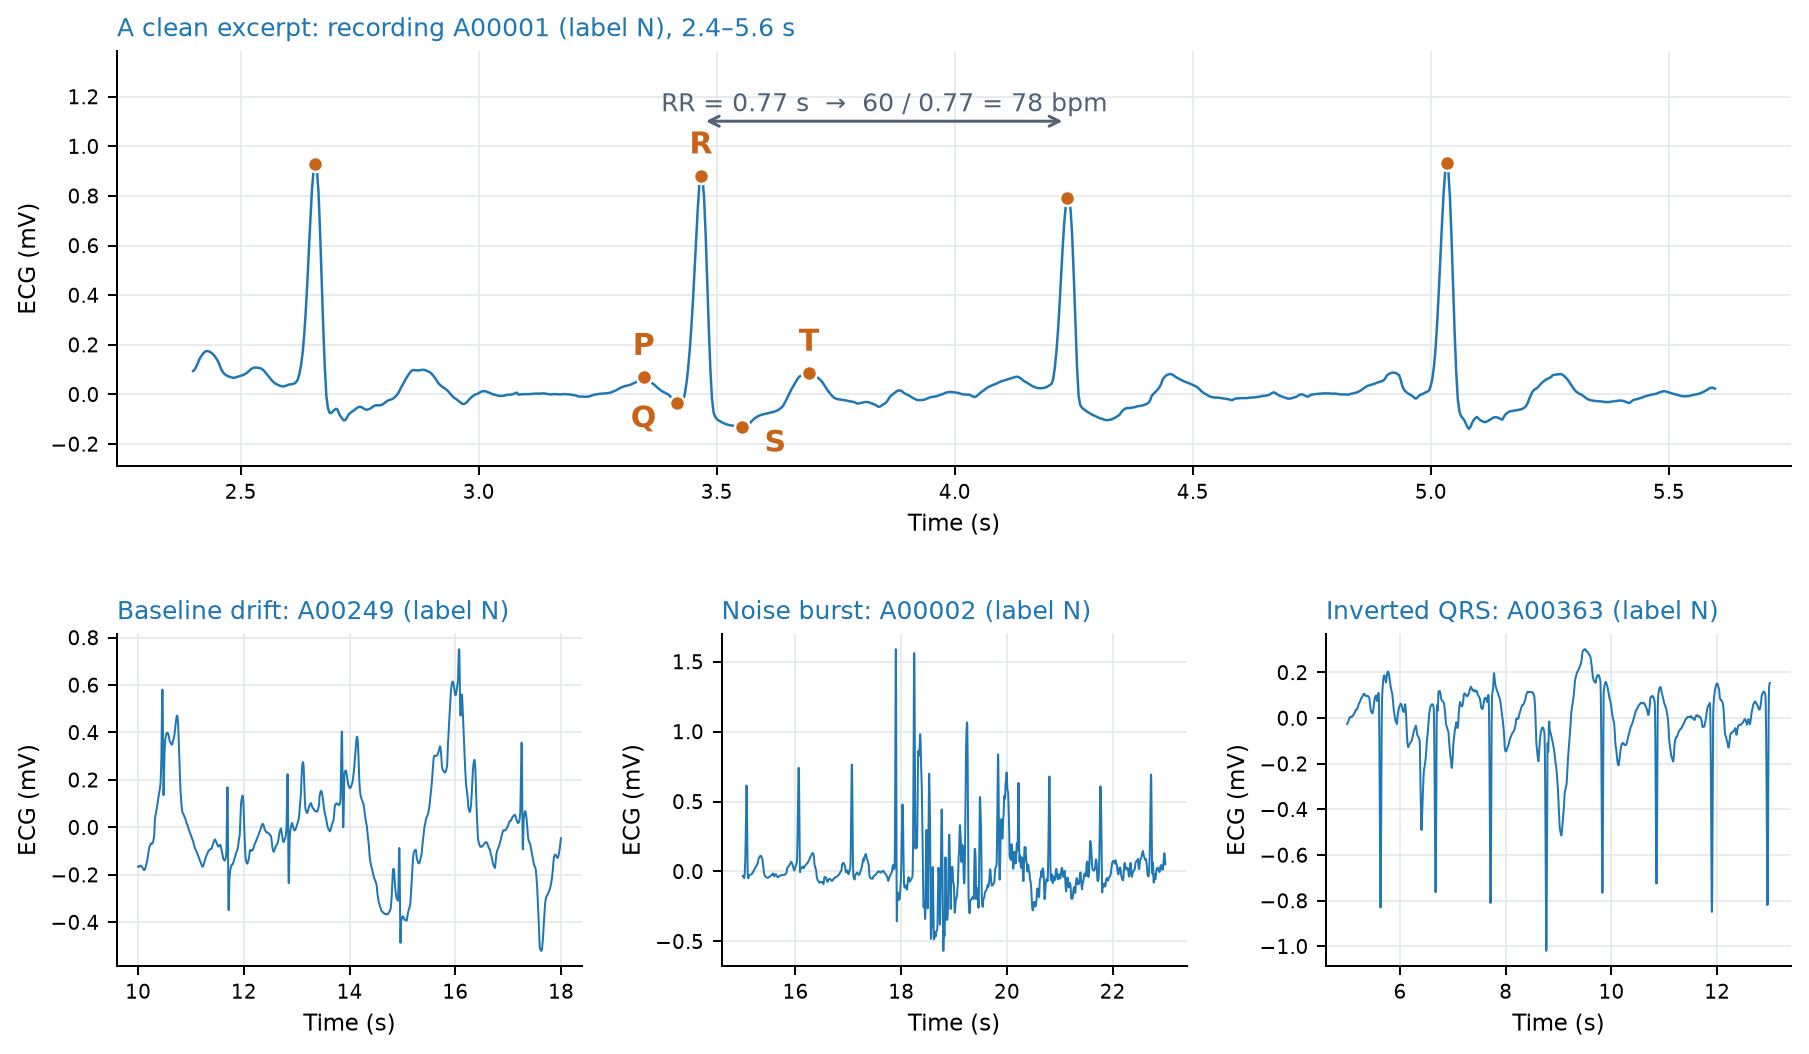
\includegraphics[width=\textwidth]{figures/ecg_anatomy.png}
  \caption{Top: three beats from a clean excerpt. One beat has its P, Q, R, S and T waves
  marked, and the RR interval is shown between two R peaks. Bottom: three things that get in the
  way, each taken from a recording labelled \texttt{N}: baseline drift, a burst of noise, and a
  QRS complex that points downwards.}
  \label{fig:anatomy}
\end{figure}

\paragraph{The waves of one beat.} Each wave corresponds to one stage of the heartbeat. The
\textbf{P wave} is small and rounded, and marks the atria contracting. The \textbf{QRS complex}
is a sharp spike, roughly \SIrange{80}{120}{\milli\second} wide and usually the tallest feature
of the beat; it marks the ventricles contracting. The Q and S waves are the small dips on either
side of the R peak. The \textbf{T wave} is broad and rounded, and marks the ventricles
recovering. In a normal beat these waves always appear in the same order, so their positions
relative to the R peak hardly vary. The wave-shape features used in Section~4 measure exactly
those positions and heights.

\paragraph{Timing.} In the top panel, the two marked R peaks are \SI{0.77}{\second} apart. That
gap is one \textbf{RR interval}, and it corresponds to a heart rate of $60 / 0.77 = 78$ beats per
minute. At rest, RR intervals are usually between \SIrange{0.6}{1.0}{\second}, which is
\SIrange{60}{100}{bpm}. The RR interval is the first feature of this lab, and it is one you can
read directly off the plot.

\paragraph{Three things that get in the way.} \emph{Baseline drift} (bottom left) comes from
breathing, body movement and changing electrode contact. It is slow, below about
\SI{0.5}{\hertz}, and the beats ride up and down on top of it, so a high voltage no longer means
a beat. A \emph{noise burst} (bottom middle) comes from movement or muscle activity. For a few
seconds the noise spikes are as tall as the R peaks. Notice that this recording is still labelled
\texttt{N}: the label describes the rhythm, not the quality of the signal. An \emph{inverted QRS}
(bottom right) depends on where the electrodes sit on the body. Here the QRS complex points
downwards, so the maximum of the signal is never the beat. Each of these would defeat a naive
rule, and Section~3 has one step to deal with each of them.

\paragraph{The recordings.} The data come from the PhysioNet/Computing in Cardiology Challenge
2017~\cite{clifford2017af, goldberger2000physionet} and are for educational use only.

\begin{center}
\singleTableRowHeight
\begin{tabular}{l p{9.2cm}}
\tableHeaderStart
\tableHCell{Item} & \tableHCell{Value} \\
\tableHeaderEnd
Device & a handheld single-lead recorder, two electrodes under the fingers \\
Recordings & 2,000: \texttt{N} 1,187, \texttt{A} 196, \texttt{O} 553, \noise\ 64 \\
Length & 9 to 60 seconds \\
Sampling rate & \SI{300}{\hertz}: time in seconds = sample index / 300 \\
Units & stored in microvolts; the notebook divides by 1,000 to plot millivolts \\
Labels & one of four rhythm classes per recording, assigned by experts: \texttt{N},
         \texttt{A}, \texttt{O} or \noise, explained below \\
\hline
\end{tabular}
\end{center}

\begin{figure}[tbp]
  \centering
  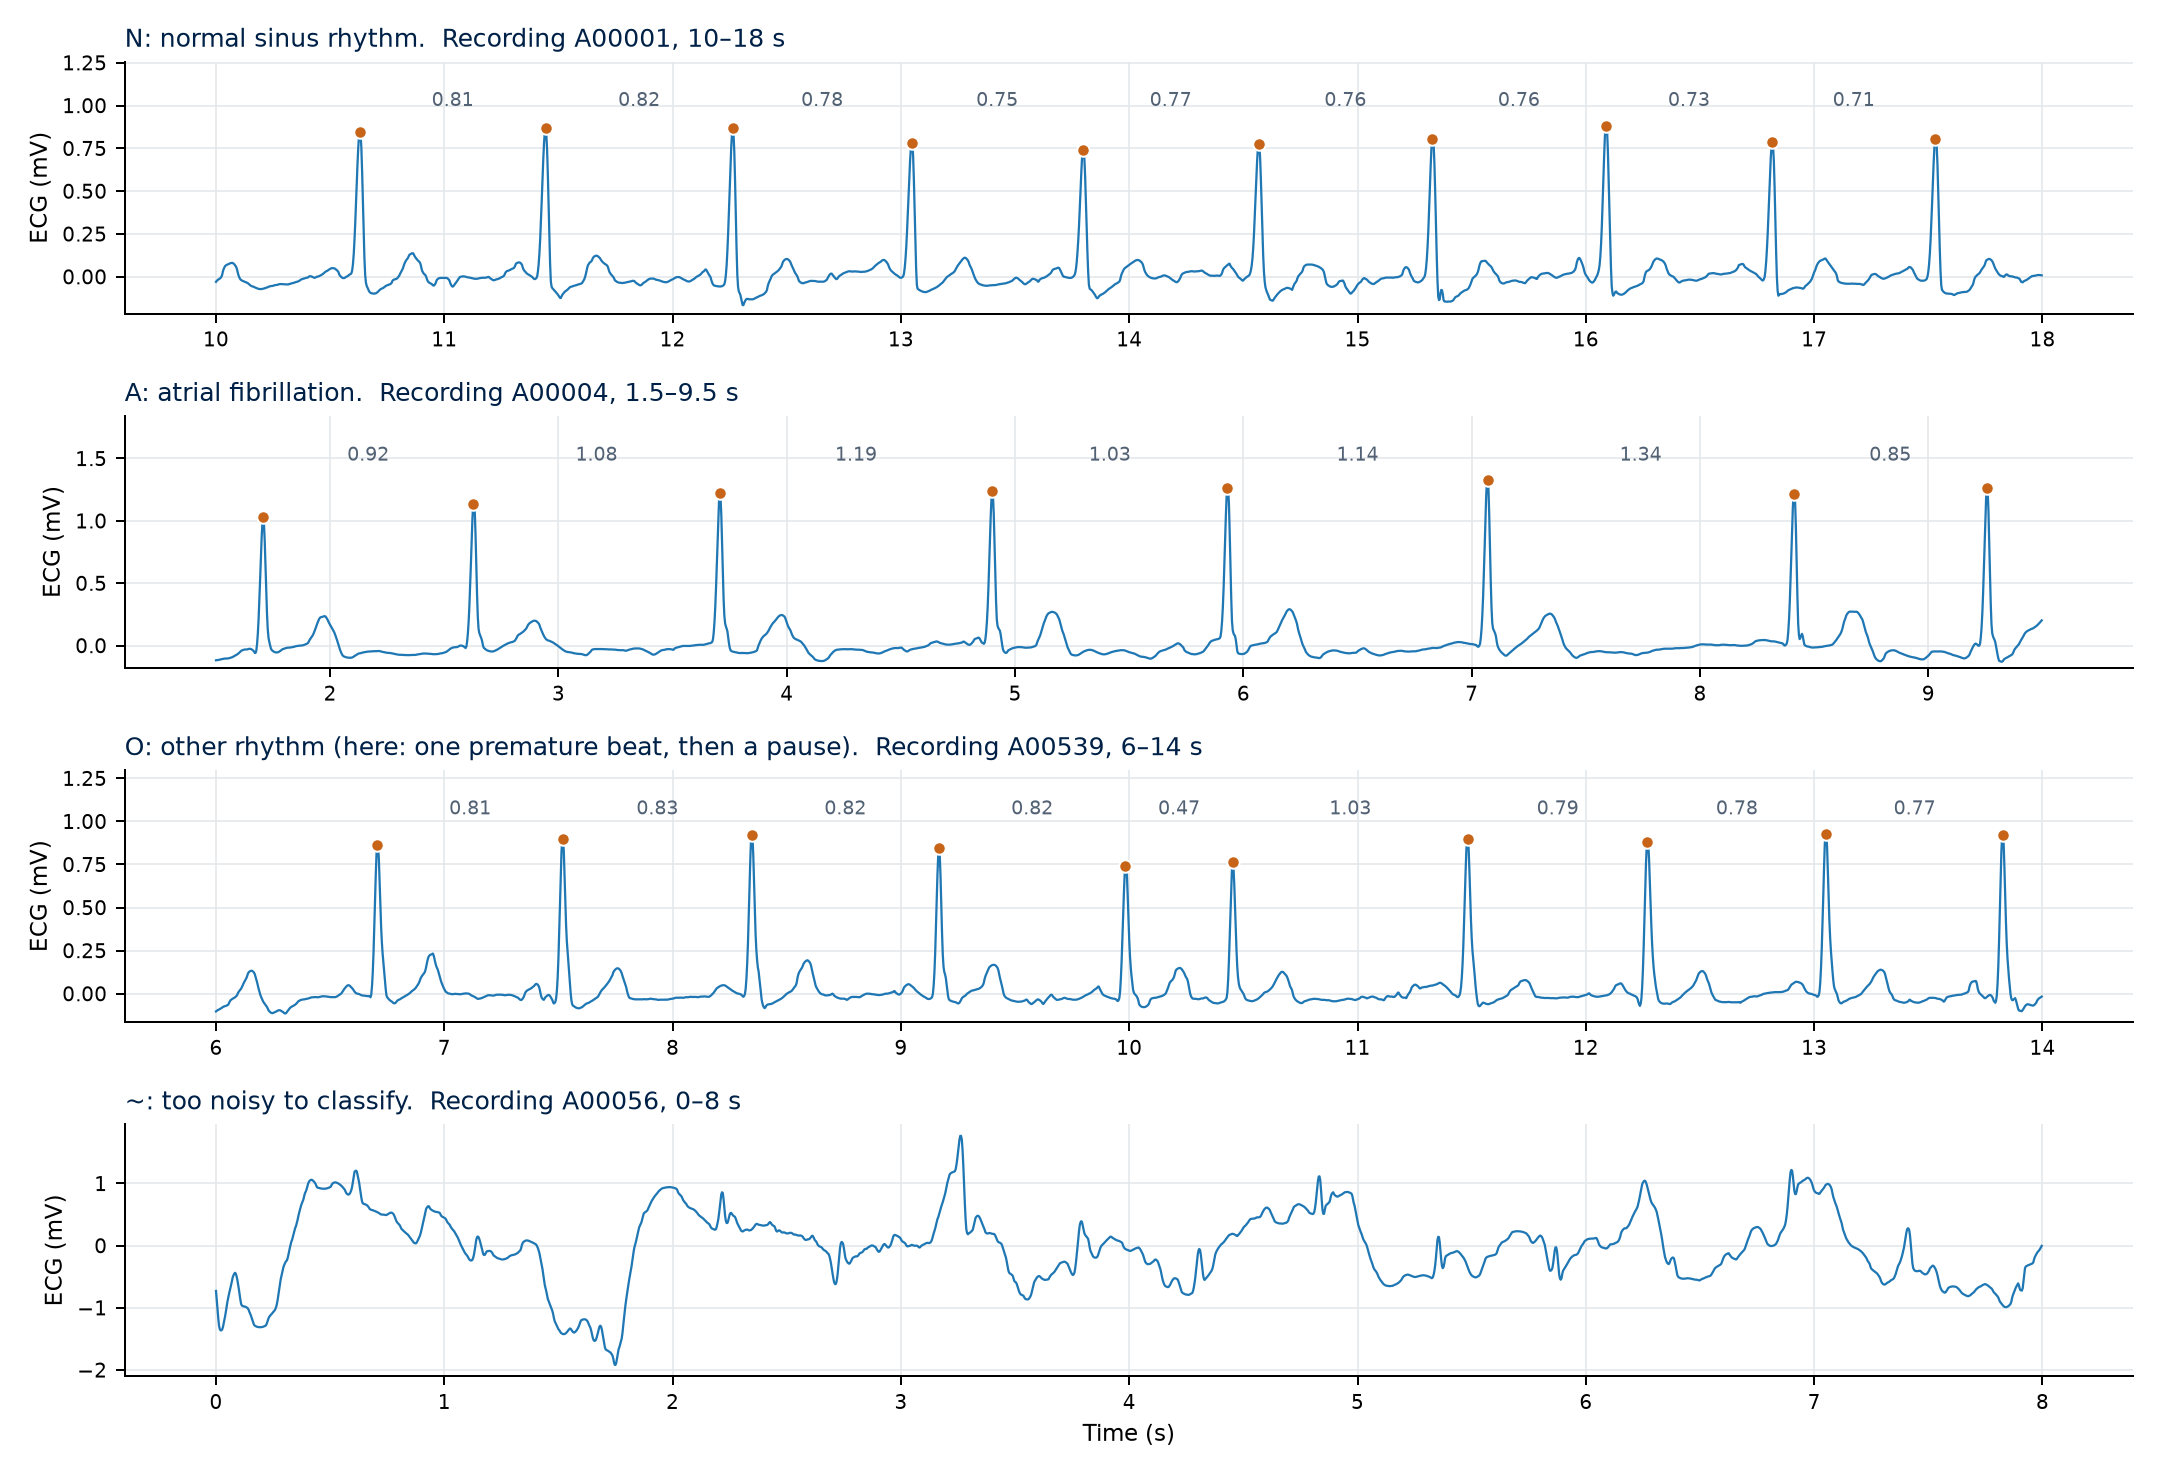
\includegraphics[width=\textwidth]{figures/labels.png}
  \caption{One recording from each class, 8 seconds each. The dots mark the beats and the
  numbers above them give the RR intervals in seconds. \texttt{N}: evenly spaced beats, each
  with a P wave. \texttt{A}: intervals that change from one beat to the next, and no P waves.
  \texttt{O}: a regular rhythm interrupted by one early beat and a pause. \noise: no beat can be
  recognised at all.}
  \label{fig:labels}
\end{figure}

\paragraph{Four heart rhythm classes.} The heart has its own pacemaker, the sinus node, which
fires at a steady rate and triggers every normal beat. The four labels describe how far a
recording's rhythm departs from that (Figure~\ref{fig:labels}):
\begin{itemize}
  \item \textbf{\texttt{N}, normal sinus rhythm.} The sinus node drives every beat. Each beat
        shows a P wave, a QRS complex and a T wave in turn, and the RR intervals change only
        gradually, for example with breathing. On the plot, the beats are evenly spaced and all
        look alike.
  \item \textbf{\texttt{A}, atrial fibrillation (AF).} The atria quiver instead of contracting,
        so there are no P waves, only a wavy baseline. The ventricles are triggered at random
        moments, so the RR intervals jump from one beat to the next: the rhythm is
        \emph{irregularly irregular}. The QRS complex itself looks normal, because the ventricles
        still contract normally. AF is the most common sustained arrhythmia and raises the risk
        of stroke, which is why being able to detect it from a wearable matters.
  \item \textbf{\texttt{O}, other rhythm.} Everything that is neither normal nor AF. This
        includes a premature beat that arrives early and is followed by a pause (as in the
        figure), runs of fast beats, a slow rhythm, and blocked conduction. It is a mixed group
        with no single appearance, which is what makes it the hardest class in Section~4.
  \item \textbf{\noise, too noisy to classify.} The signal is so corrupted that no rhythm can be
        read from it.
\end{itemize}
A label describes the rhythm of the \emph{whole} recording. Apart from \noise, it says nothing
about the quality of the signal, and it does not promise that every beat is normal: an
\texttt{N} recording can still contain an artefact or a single premature beat.

\paragraph{Task 1.} The notebook shows you six excerpts from \texttt{N} recordings. In each
one, ten consecutive wave points spanning two beats are marked with numbered dots. The first
excerpt is labelled for you as the worked example (P Q R S T P Q R S T). The other five each
start at a different point in the cycle, so you have to read each dot from the shape of the
signal rather than from its position in the sequence. \emph{Submit:} the ten letters for each of
the five diagrams, in order, with the notebook's check passed. The check tells you which dots
are wrong, but never prints the answer.

\paragraph{Carry forward.} The R peak is our landmark, and the RR interval is our first
feature. An \texttt{N} label does not promise a clean signal: drift, noise bursts and inverted
beats are all present in this dataset, and every step that follows has to survive them.


% ____________________________________________________________________________
\needspace{10\baselineskip}
\section{Measuring rhythm from ECG signals}
\nb{Section 2}

\paragraph{What this section is for.} Section~1 ended with a warning: the R peak is our
landmark, but in a wearable recording it sits on a drifting baseline, inside noise bursts, and
sometimes upside down, so picking the highest points of the signal is not enough. This section
shows what we want \emph{out} of such a signal before Section~3 builds the detector that
gets it. It walks the whole route once, on three real recordings of the dataset, one of each
rhythm: raw signal, the beats a detector finds in it, the intervals between those beats, and the
handful of numbers that describe the rhythm. To do that without a detector of our own yet, the
beats are found by an established library, NeuroKit2, which plays the part that your detector
will play from Section~3 on. Everything after the beats is arithmetic, and you write that
arithmetic in Task~2.

\paragraph{What people measure.} Clinicians and wearables describe the rhythm of the heart by
the \emph{times} of its beats, not by the shape of the waves. Three quantities cover most of what
is reported. The RR intervals are the gaps between consecutive R peaks. Their average gives the
heart rate, the number every watch shows. How much they change from one beat to the next is
heart rate variability (HRV), of which RMSSD is the most used measure and the one that separates
atrial fibrillation from normal rhythm. Figure~\ref{fig:rhythm} shows all three on the
\texttt{N}, \texttt{A} and \texttt{O} recordings of Figure~\ref{fig:labels}, and then heart rate
and RMSSD for every recording in the dataset. The two numbers you compute here, heart rate and
RMSSD, are the ones you will check and chase through the rest of the lab: every detector step in
Section~3 is judged by how much it moves them, and Section~4 feeds them, with 23 relatives, to
the classifier.

\begin{figure}[tbp]
  \centering
  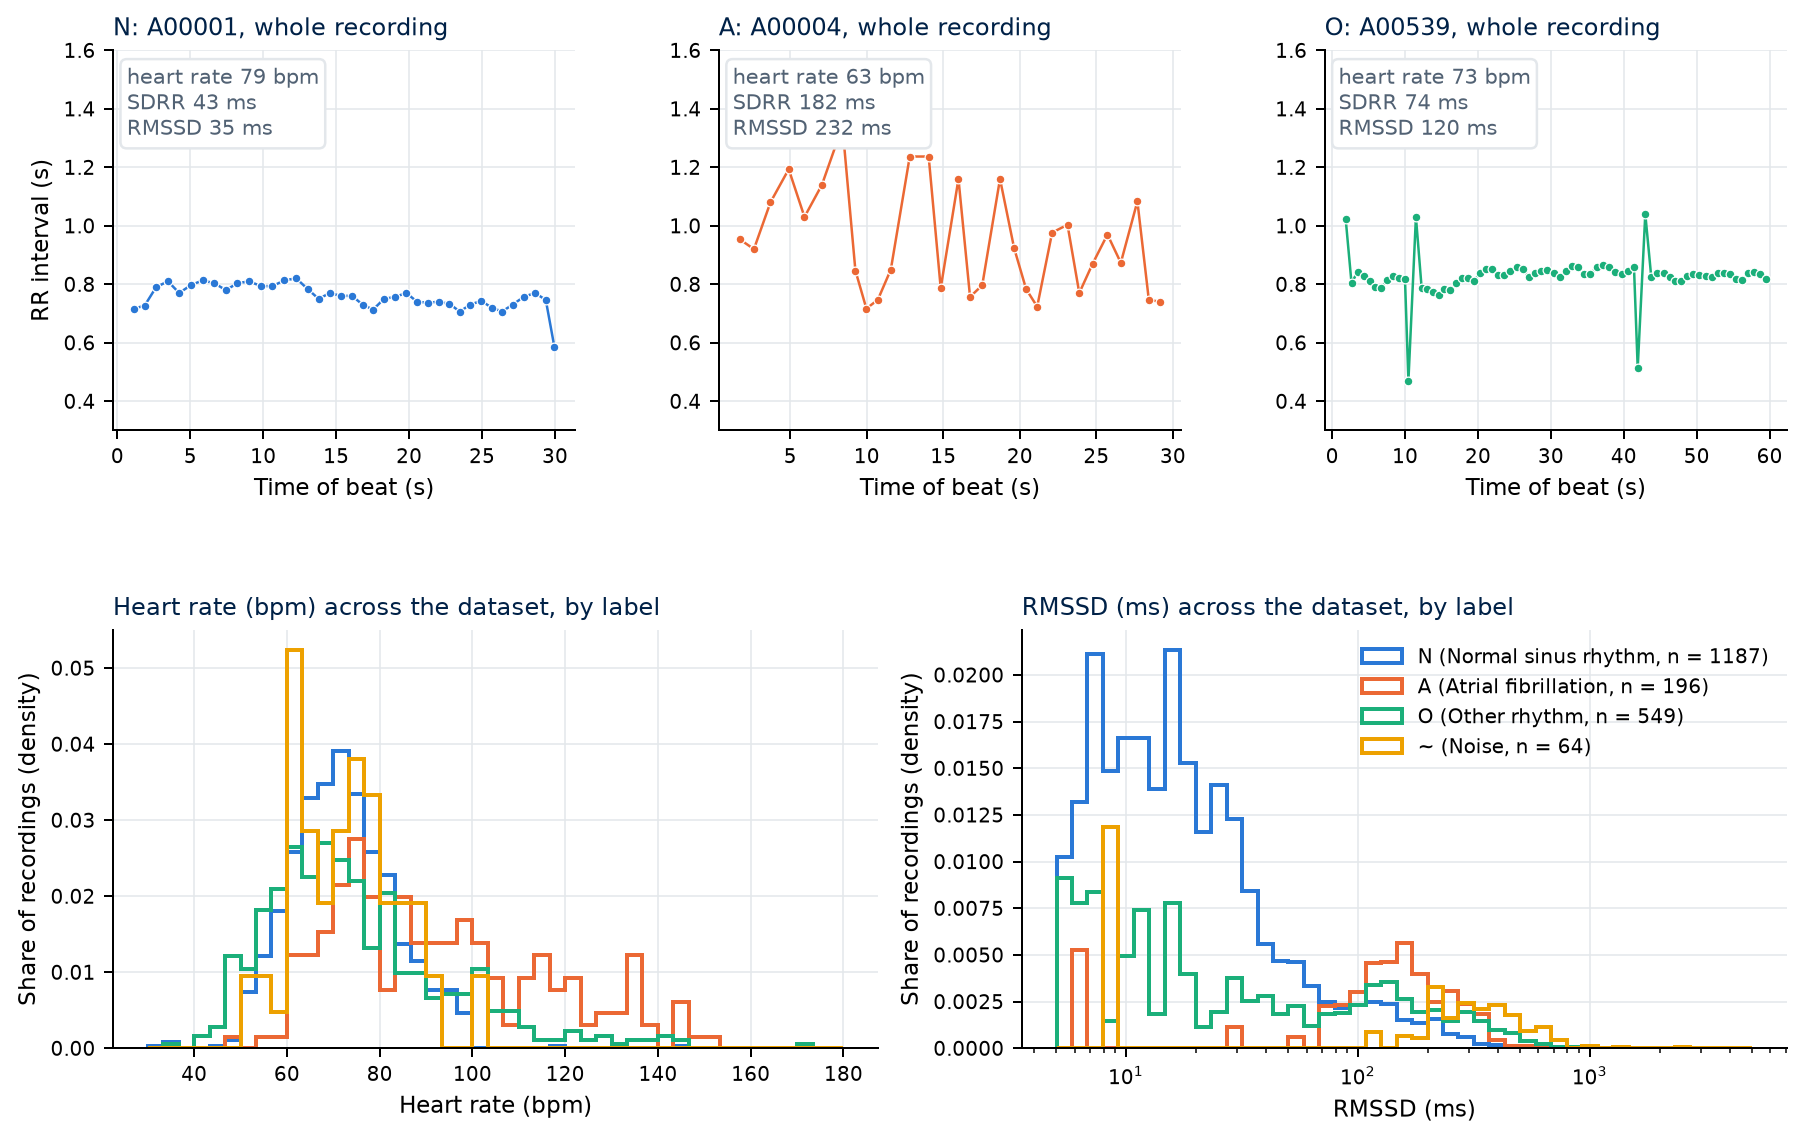
\includegraphics[width=\textwidth]{figures/rhythm_features.png}
  \caption{Top: the RR intervals of the \texttt{N}, \texttt{A} and \texttt{O} recordings of
  Figure~\ref{fig:labels}, over the whole recording, with the heart rate, SDRR and RMSSD
  calculated from them. Bottom: heart rate and RMSSD (log axis) for every recording in the
  dataset, by label. Medians: \texttt{N} \SI{71}{bpm} and \SI{49}{\milli\second}; \texttt{A}
  \SI{89}{bpm} and \SI{188}{\milli\second}; \texttt{O} \SI{71}{bpm} and \SI{181}{\milli\second};
  \noise\ \SI{73}{bpm} and \SI{394}{\milli\second}. Beats found by NeuroKit2.}
  \label{fig:rhythm}
\end{figure}

\paragraph{From beats to intervals.} From $K$ beats at sample indices $s_1, \dots, s_K$ and
sampling rate $f_s$:
\begin{align*}
  t_k &= s_k / f_s && \text{beat times (s)}\\
  RR_k &= t_{k+1} - t_k && \text{RR intervals (s), } K-1 \text{ of them.}
\end{align*}
Plotting $RR_k$ against time (Figure~\ref{fig:rhythm}, top) is the quickest way to see a
rhythm. The \texttt{N} recording is a nearly flat line that drifts slowly. The \texttt{A}
recording jumps from one interval to the next. The \texttt{O} recording is flat except for one
short interval followed by one long one: the premature beat and its pause.

\paragraph{Heart rate.} Two versions are in use:
\begin{align*}
  HR_k &= 60 / RR_k && \text{instantaneous heart rate (bpm)}\\
  HR_\text{period} &= 60\,(K-1) / (t_K - t_1) = 60 / \overline{RR} && \text{rate over the period (bpm).}
\end{align*}
The period rate is the number a wearable shows. All three recordings in the figure are in the
resting range, 63 to \SI{79}{bpm}, and the bottom-left panel shows the same across the dataset:
the four labels overlap heavily. Heart rate alone does not tell the rhythms apart.

\paragraph{Heart rate variability.} With the $N = K-1$ intervals in milliseconds, the two most
used time-domain features~\cite{taskforce1996hrv} are
\[
  \text{SDRR} = \sqrt{\frac{1}{N-1}\sum_{k=1}^{N}\left(RR_k - \overline{RR}\right)^2},
  \qquad
  \text{RMSSD} = \sqrt{\frac{1}{N-1}\sum_{k=1}^{N-1}\left(RR_{k+1} - RR_k\right)^2}.
\]
SDRR is the spread of the intervals around their mean; RMSSD is the typical change from one
interval to the next. They answer different questions. A slow drift of the rate, as in the
\texttt{N} recording, gives some SDRR (\SI{43}{\milli\second}) and less RMSSD
(\SI{35}{\milli\second}). Abrupt changes, as in atrial fibrillation, give a lot of both
(182 and \SI{232}{\milli\second}). One premature beat, as in the \texttt{O} recording, moves
SDRR somewhat (\SI{74}{\milli\second}) and RMSSD a lot (\SI{120}{\milli\second}), because the
short interval and the long one after it are two large successive differences. In the
bottom-right panel RMSSD separates \texttt{N} from \texttt{A} well, with medians of 49 and
\SI{188}{\milli\second}. \texttt{O} overlaps both, which is why it is the hardest class in
Section~4, and \noise\ is largest of all, because wrongly placed beats look exactly like an
irregular rhythm. Two cautions: call SDRR \emph{SDNN} only when the intervals are confirmed to be
normal-to-normal, and treat values from recordings this short as descriptive, not as a clinical
assessment.

\paragraph{More of the same.} NeuroKit2's \texttt{hrv\_time} returns 25 time-domain HRV
features, all variations on the ideas above (Table~\ref{tab:hrv}). Section~4 uses all of them,
and they carry most of the classifier's performance.

\begin{table}[htbp]
\centering
\singleTableRowHeight
\small
\begin{tabular}{p{4.6cm} p{9cm}}
\tableHeaderStart
\tableHCell{What it measures} & \tableHCell{Features (NeuroKit2 names)} \\
\tableHeaderEnd
The typical interval, i.e.\ the rate & MeanNN, MedianNN, MinNN, MaxNN \\
Spread of the intervals & SDNN (our SDRR), CVNN, MadNN, MCVNN, IQRNN, Prc20NN, Prc80NN;
  SDANN1/2/5 and SDNNI1/2/5 over 1, 2 and 5-minute segments, undefined on recordings this short \\
Change from one interval to the next & RMSSD, SDSD, CVSD, pNN50 and pNN20 (share of successive
  differences above 50 and \SI{20}{\milli\second}), SDRMSSD \\
Shape of the RR histogram & HTI, TINN \\
\hline
\end{tabular}
\caption{The 25 time-domain HRV features of \texttt{hrv\_time}, grouped by what they measure
(the \texttt{HRV\_} prefix of each name is dropped).}
\label{tab:hrv}
\end{table}

\paragraph{Task 2.} NeuroKit2 finds the beats of a recording, and the RR sequence
is the differences between consecutive beat times. Implement \texttt{rhythm\_features}, which
turns an RR sequence into the heart rate, SDRR and RMSSD using the formulas above. The notebook
runs it on the three recordings of Figure~\ref{fig:rhythm} and checks every value against
NeuroKit2's own \texttt{hrv\_time} on the same beats. \emph{Deliver:} the function with the
check passed, and the three-row table it prints.

\begin{tcolorbox}[breakable, title=Specification: \texttt{rhythm\_features(rr\_s)}, colback=white, colframe=black!60]
\begin{description}[leftmargin=*, itemsep=2pt, font=\bfseries]
  \item[Given] \texttt{rr\_s}, a 1-D NumPy array of RR intervals in seconds, in time order: about 40 values for a \SI{30}{\second} recording, typically between 0.6 and \SI{1.2}{\second}, built from NeuroKit2's beats.
  \item[You may use] NumPy only: the mean, the sample standard deviation, differences between neighbouring values, the square root.
  \item[Return] a tuple of three floats \texttt{(heart\_rate\_bpm, sdrr\_ms, rmssd\_ms)}: $60 / \overline{RR}$; the sample standard deviation of the intervals in ms; the square root of the mean of the squared successive differences in ms, squared before averaging.
  \item[Checked by] NeuroKit2's \texttt{hrv\_time} on the same beats, for three recordings, to six significant figures.
\end{description}
\end{tcolorbox}

\paragraph{Carry forward.} Heart rate is $60 / \overline{RR}$; RMSSD is the root mean square of
the successive differences, and you have coded both. Both need the beat times, and RMSSD needs
every one of them to be right, which is where Section~3 starts.


% ____________________________________________________________________________
\needspace{10\baselineskip}
\section{Extracting rhythm features from noisy raw signals}
\nb{Section 3}

In this section you will learn to extract two rhythm features,
heart rate and RMSSD, from noisy raw ECG signals. The route is always the same: find the beats,
then pass their times to the \texttt{rhythm\_features} you wrote in Task~2. The work is
finding the beats, and we go through it in four steps:
\begin{enumerate}[leftmargin=*, itemsep=2pt]
  \item We use NeuroKit2, an established ECG library, as a reference beat detector
        (Section~\ref{sec:reference}).
  \item We implement a naive peak-finding beat detector: a threshold on the raw signal
        (Section~\ref{sec:naive}).
  \item We implement a detector that searches for the QRS complex instead of peaks, in three
        steps: filter, emphasise fast changes, locate the R peak (Section~\ref{sec:qrs}).
  \item We add median imputation, which uses the rhythm itself to drop extra beats and fill in
        missed ones, and so corrects the HRV estimate (Section~\ref{sec:impute}).
\end{enumerate}
At steps 2 to 4 we measure how well our detector agrees with the NeuroKit2 reference: its beats,
and the heart rate and RMSSD computed from them, across every recording in the dataset. The
settings are teaching choices for \SI{300}{\hertz} data, not a validated clinical detector.



\subsection{NeuroKit2: a reference beat detector}
\label{sec:reference}
\nb{3.1}

\paragraph{The NeuroKit2 reference.} NeuroKit2~\cite{makowski2021neurokit2} is an open-source library
used across research and industry to turn an ECG into beats and features, and its default
pipeline (\texttt{ecg\_clean}, then \texttt{ecg\_peaks}) belongs to the same family as the
detector you build in this section: filter, emphasise the fast QRS, threshold, place the beat. It is the
\emph{NeuroKit2 reference} for this section, as the notebook calls it: its beats for
every recording, with no correction, and the heart rate and RMSSD from them (the circles in
Figure~\ref{fig:naive}). Every step you add is a step the library also takes, so closing the
gap to it is how you find out what sits inside a library call, and where the practice has
choices. Two things to keep in mind. The dataset labels rhythms, not beats, so there is no
ground truth here: the reference is an established pipeline, not the truth, and a gap to it
means \emph{different}. And both detectors can make the same mistake, which no score can see.

\paragraph{The evaluation.} In the notebook, each step is one short function that you write from
its description (Tasks~4A to 4D), with its setting next to it and a self-check against a
reference; a detector is the set of functions so far, kept in a dictionary:
\texttt{steps\_naive}, then \texttt{steps\_4a = \{**steps\_naive, "filter": bandpass\}}, and
so on. \texttt{bench.score(name, steps)} runs a detector on every recording, prints three
scores against the NeuroKit2 reference, enters it on a leaderboard and plots it next to the reference:
\begin{itemize}
  \item \textbf{beat agreement}: beats paired with a reference beat within
        $\pm$\SI{100}{\milli\second}, as $2 \times \text{matched} / (\text{ours} + \text{reference})$;
        1 when every beat pairs;
  \item \textbf{heart rate error}: $|$ours $-$ reference$|$ per recording, summarised by the MAE
        (mean absolute error, the typical error) and the P95 (the error only the worst 5\% of
        recordings exceed);
  \item \textbf{RMSSD error}: the same, in ms.
\end{itemize}

\subsection{A naive peak-finding detector}
\label{sec:naive}
\nb{3.2, Task 3}

The QRS is the fastest and usually the tallest event of
each beat (Section~1), so a peak finder emphasises fast changes, thresholds the result, and
places one beat in each region above the threshold, at the R peak. Section~\ref{sec:qrs} builds it in
three steps: filter out drift and fast noise; differentiate, square
and integrate, so that each QRS gives one bump; locate the R peak inside each bump. On the
recording in Figure~\ref{fig:recipe} (Section~\ref{sec:impute}) it finds 34 beats: 33 real ones, an artefact at
\SI{1.0}{\second}, and none at \SI{25.8}{\second}, where the QRS was too small to cross the
threshold.

\paragraph{Task 3: detector v1.} The simplest peak finder is the threshold alone,
and it is the first version of your detector. Write
\texttt{naive\_beats}, which takes an ECG signal and a threshold in millivolts and returns the
sample index of each beat: one beat per region where the signal is above the threshold, at the
region's highest sample. The notebook checks it on an invented signal and against a reference on
your recording, shows your beats with the threshold next to NeuroKit2's, and turns them into
heart rate and RMSSD with your \texttt{rhythm\_features}: your first features extracted end to
end. \emph{Deliver:} the function with both checks passed, and the plot.

\begin{tcolorbox}[breakable, title=Specification: \texttt{naive\_beats(signal, threshold)}, colback=white, colframe=black!60]
\begin{description}[leftmargin=*, itemsep=2pt, font=\bfseries]
  \item[Given] \texttt{signal}, a 1-D NumPy array of one ECG lead in mV, one value per sample at
        $f_s = \SI{300}{\hertz}$ (9,000 samples for \SI{30}{\second}); \texttt{threshold}, one number in
        mV. The signal rises above the threshold at every QRS complex, and sometimes at a tall T wave
        or an artefact; each crossing is a run of consecutive samples above it, a \emph{region}.
  \item[You may use] NumPy only: comparisons, padding, differences between neighbouring values,
        the positions of non-zero values, slicing, and the position of a maximum.
  \item[Return] a 1-D integer array of sample indices, one per region, at the region's highest
        sample, in increasing order; empty if nothing crosses. Time in seconds = index / $f_s$.
  \item[Checked by] the invented signal \texttt{[0, 1, 3, 1, 0, 0, 2, 5, 2, 0, 1, 0]} with
        threshold 1.5, which must give \texttt{[2, 7]}; and a reference implementation on your
        recording.
\end{description}
\end{tcolorbox}

\paragraph{Detector v1 on the benchmark.} Your Task~3 rule, with one change: amplitude differs between
people, electrodes and recordings, so the threshold is relative, 20\% of the recording's maximum
in its middle half, rather than a value in millivolts. Each region above the threshold gives one
beat, at its highest point. On \texttt{A00001} this finds most beats; on \texttt{A00726} it finds 54 beats
where there are 34, because P and T waves and a baseline swing also cross the threshold
(Figure~\ref{fig:naive}, and the top panel of Figure~\ref{fig:step1}). Every later step keeps
this threshold rule and changes one thing before it.

\begin{figure}[htbp]
  \centering
  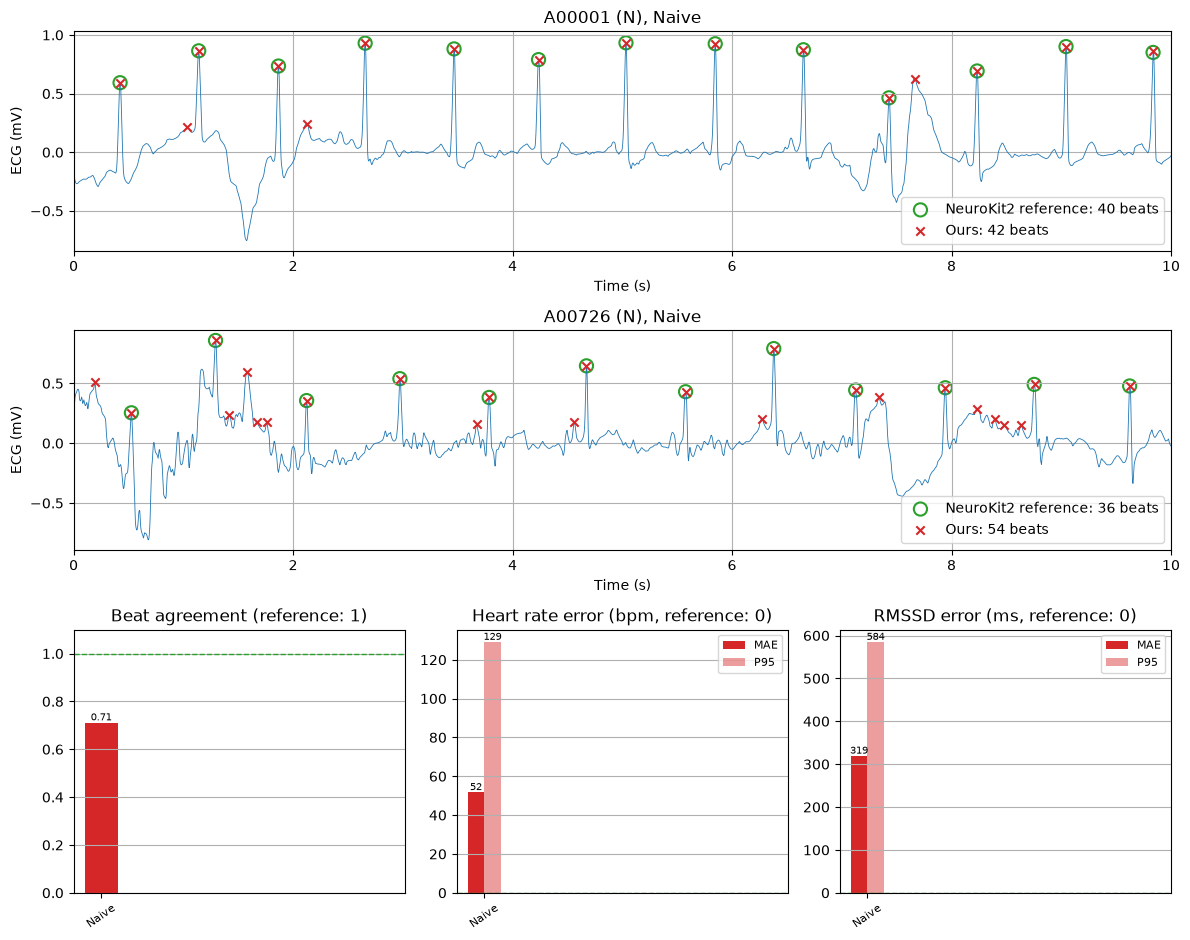
\includegraphics[width=0.85\textwidth]{figures/naive.png}
  \caption{The naive detector (crosses) and the NeuroKit2 reference (circles) on \texttt{A00001} and
  \texttt{A00726}, and its scores across the dataset.}
  \label{fig:naive}
\end{figure}

\subsection{A beat detector that searches for the QRS complex}
\label{sec:qrs}
\nb{3.3, Tasks 4A--4C}

In this subsection we develop a QRS-searching detector, detector v2. Instead of looking for
tall points, it looks for the \emph{rapid changes} that characterise the QRS complex: the
sharpest edges in every beat, whatever their height or sign. It grows out of your naive
detector v1 in three steps, in the style of the QRS detector of Pan and
Tompkins~\cite{pan1985qrs}:
\begin{enumerate}[leftmargin=*, itemsep=2pt]
  \item \textbf{Denoise} with a band-pass filter, so that baseline drift and fast noise do not
        cross the threshold (Task~4A).
  \item \textbf{Differentiate, square and integrate}, so that the signal measures speed rather
        than height and each QRS complex becomes one bump (Task~4B).
  \item \textbf{Locate the R peak} inside each bump, back on the ECG (Task~4C).
\end{enumerate}
Each step is introduced by the \emph{problem} the previous detector still has, the \emph{idea}
that addresses it, and the \emph{caveats} it brings, and each is scored against the NeuroKit2
reference across all 1,996 recordings, so that you see what it buys and what it costs. The
figures follow recording \texttt{A00726} through every step. Getting close to an established
library with a detector you built yourself is how you find out what the industry has been doing
for decades to get features out of ECG signals.

\subsubsection{Step 1: denoise with a band-pass filter}
\nb{Task 4A}
\emph{Problem:} the baseline drifts and fast noise rides on the signal; both can cross a
threshold. \emph{Idea:} keep the band where the ECG waves live, \SIrange{0.5}{40}{\hertz}, the
bandwidth that monitoring ECGs have used for decades~\cite{kligfield2007ecg}: below
\SI{0.5}{\hertz} sits baseline wander from breathing and electrode movement, above
\SI{40}{\hertz} sit muscle noise and mains hum. A Butterworth filter applied forwards and
backwards keeps the band without shifting any peak.
\emph{Caveats:} the band is an assumption; real features outside it are distorted, and a
corrupted segment stays corrupted.

\begin{figure}[htbp]
  \centering
  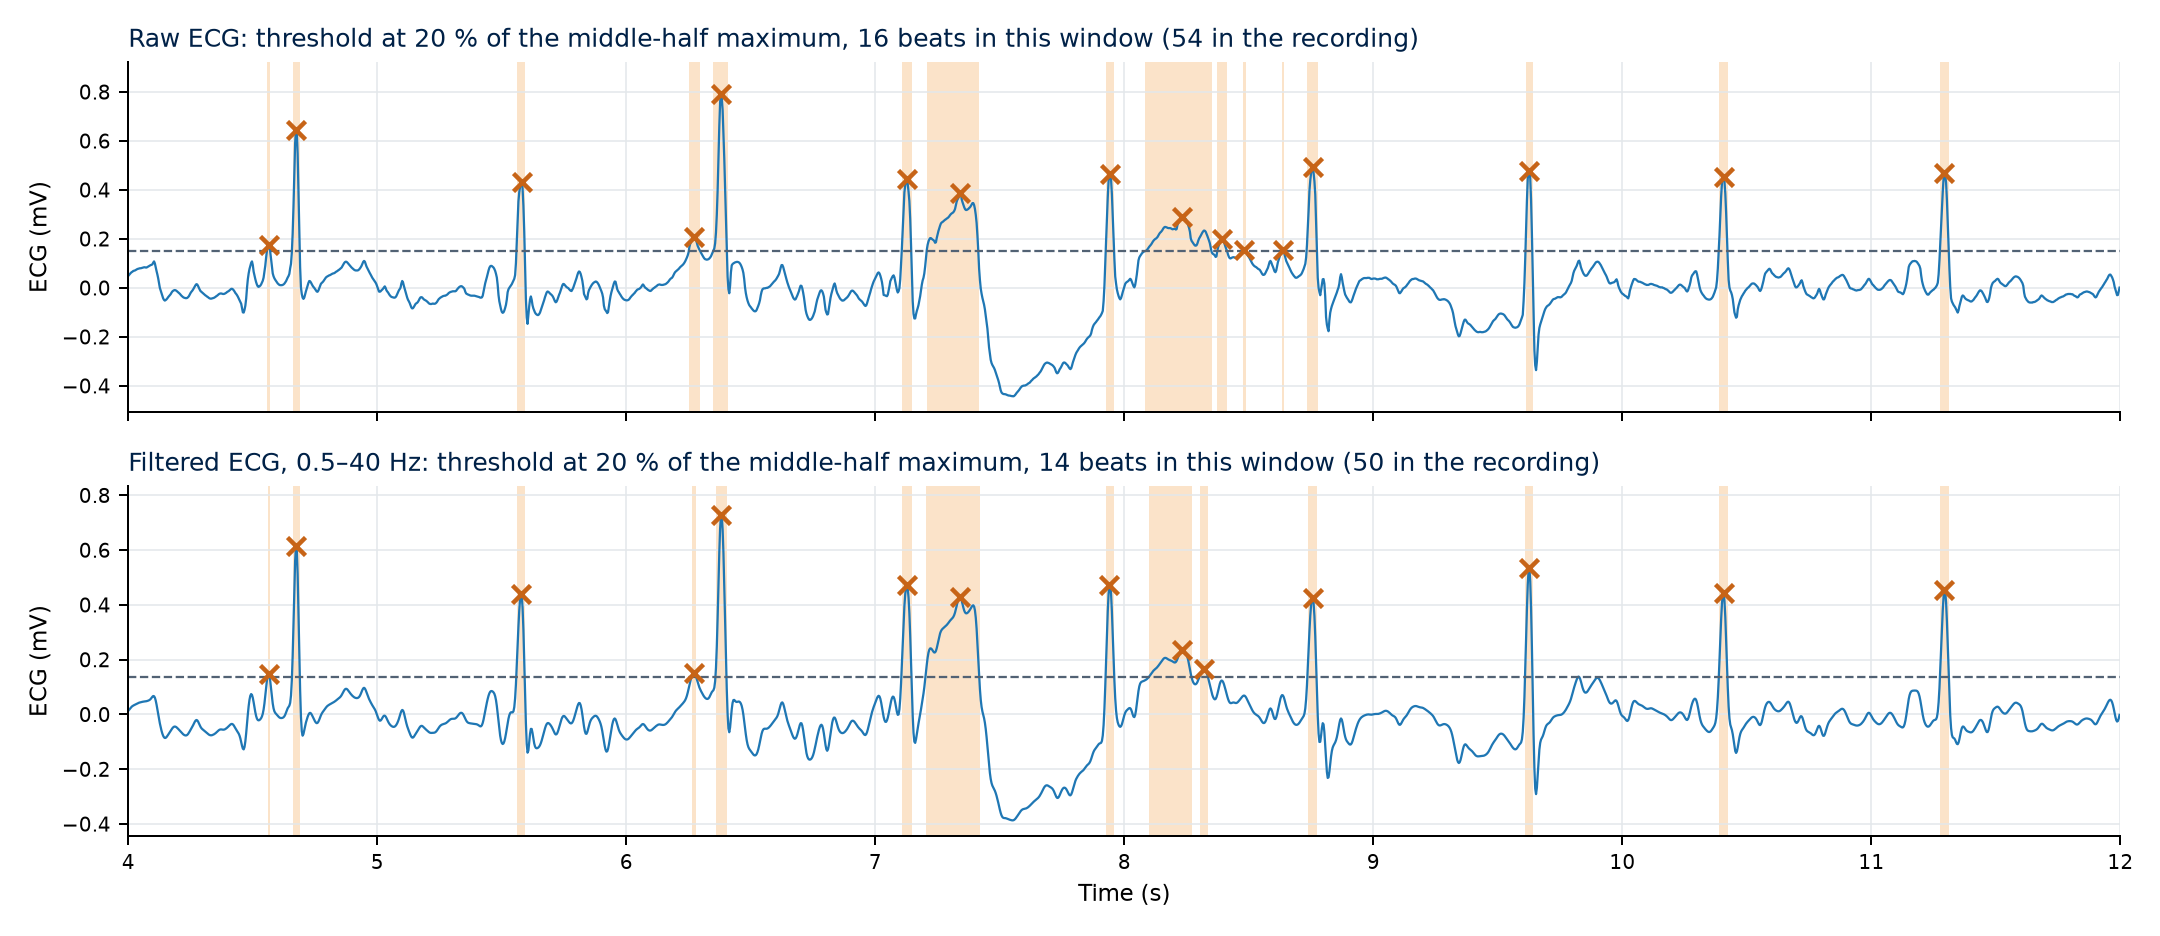
\includegraphics[width=\textwidth]{figures/step1_filter.png}
  \caption{Step 1 on \texttt{A00726}, 4 to \SI{12}{\second}: the naive threshold rule on the raw
  ECG (top) and on the filtered ECG (bottom), with the regions above the threshold shaded and
  the beat each region gives. The baseline is flatter and two P-wave crossings are gone, but the
  swing at \SIrange{7}{8}{\second} still crosses the threshold.}
  \label{fig:step1}
\end{figure}

\paragraph{What it bought.} A cleaner signal, but not a better score: beat agreement 0.71 to
0.72, heart rate MAE 51.7 to \SI{52.6}{bpm}. The filter does what it is for: the baseline is
flatter and the small high-frequency noise outside the band is gone, which is why two P-wave
crossings disappear in Figure~\ref{fig:step1}. But the threshold is still a test of
\emph{height}, and the things that fool it most, T waves, slow swings and inverted QRS
complexes, are ECG and live inside the band, so the filter cannot remove them. The filter
comes first because of step 2: once height is turned into speed, any fast noise left in the
signal is emphasised just as much as a QRS. On this dataset, which has little fast noise, that
is worth little (removing the filter from the full detector barely changes the scores); on a
noisier wearable it would be worth more.

\paragraph{Task 4A.} Write \texttt{bandpass}: design the filter with
\texttt{butter} (order 4, the band \SIrange{0.5}{40}{\hertz}, \texttt{fs=FS}, second-order
sections) and apply it with \texttt{sosfiltfilt}. \emph{Deliver:} the function with the check
passed, and its leaderboard line.

\begin{tcolorbox}[breakable, title=Specification: \texttt{bandpass(x)}, colback=white, colframe=black!60]
\begin{description}[leftmargin=*, itemsep=2pt, font=\bfseries]
  \item[Given] \texttt{x}, a 1-D array, the whole raw recording in mV at \SI{300}{\hertz}, with baseline drift and fast noise on it; the settings \texttt{low\_hz} and \texttt{high\_hz} (0.5 and 40) above the function.
  \item[You may use] SciPy's \texttt{butter} and \texttt{sosfiltfilt}, imported at the top of the cell; their documentation gives the arguments.
  \item[Return] a float array of the same length: the ECG through a fourth-order Butterworth band-pass between the two cutoffs, as second-order sections, applied forwards and then backwards so that no peak is shifted in time.
  \item[Checked by] a reference implementation on your recording.
\end{description}
\end{tcolorbox}

\subsubsection{Step 2: differentiate, square, integrate}
\nb{Task 4B}
\emph{Problem:} height is a poor clue; a tall T wave can be as high as the R peak, and some
QRS complexes point down. \emph{Idea:} the QRS is different because it is \emph{fast}
(Figure~\ref{fig:step2}). Differentiate, $d[n] = x[n] - x[n-1]$, to measure speed: large at
the sharp QRS edges, small on slow waves. Square, so that both signs count and large values
grow much more than small ones. Integrate with a centred moving average about one QRS wide
(\SI{120}{\milli\second}, 37 samples), merging the spikes of one beat into one bump. Only
together do the three give the threshold one bump per beat, so they are one step.
\emph{Caveats:} a strong noise spike is emphasised just as much as a QRS, and the bump is smeared
in time.

\begin{figure}[htbp]
  \centering
  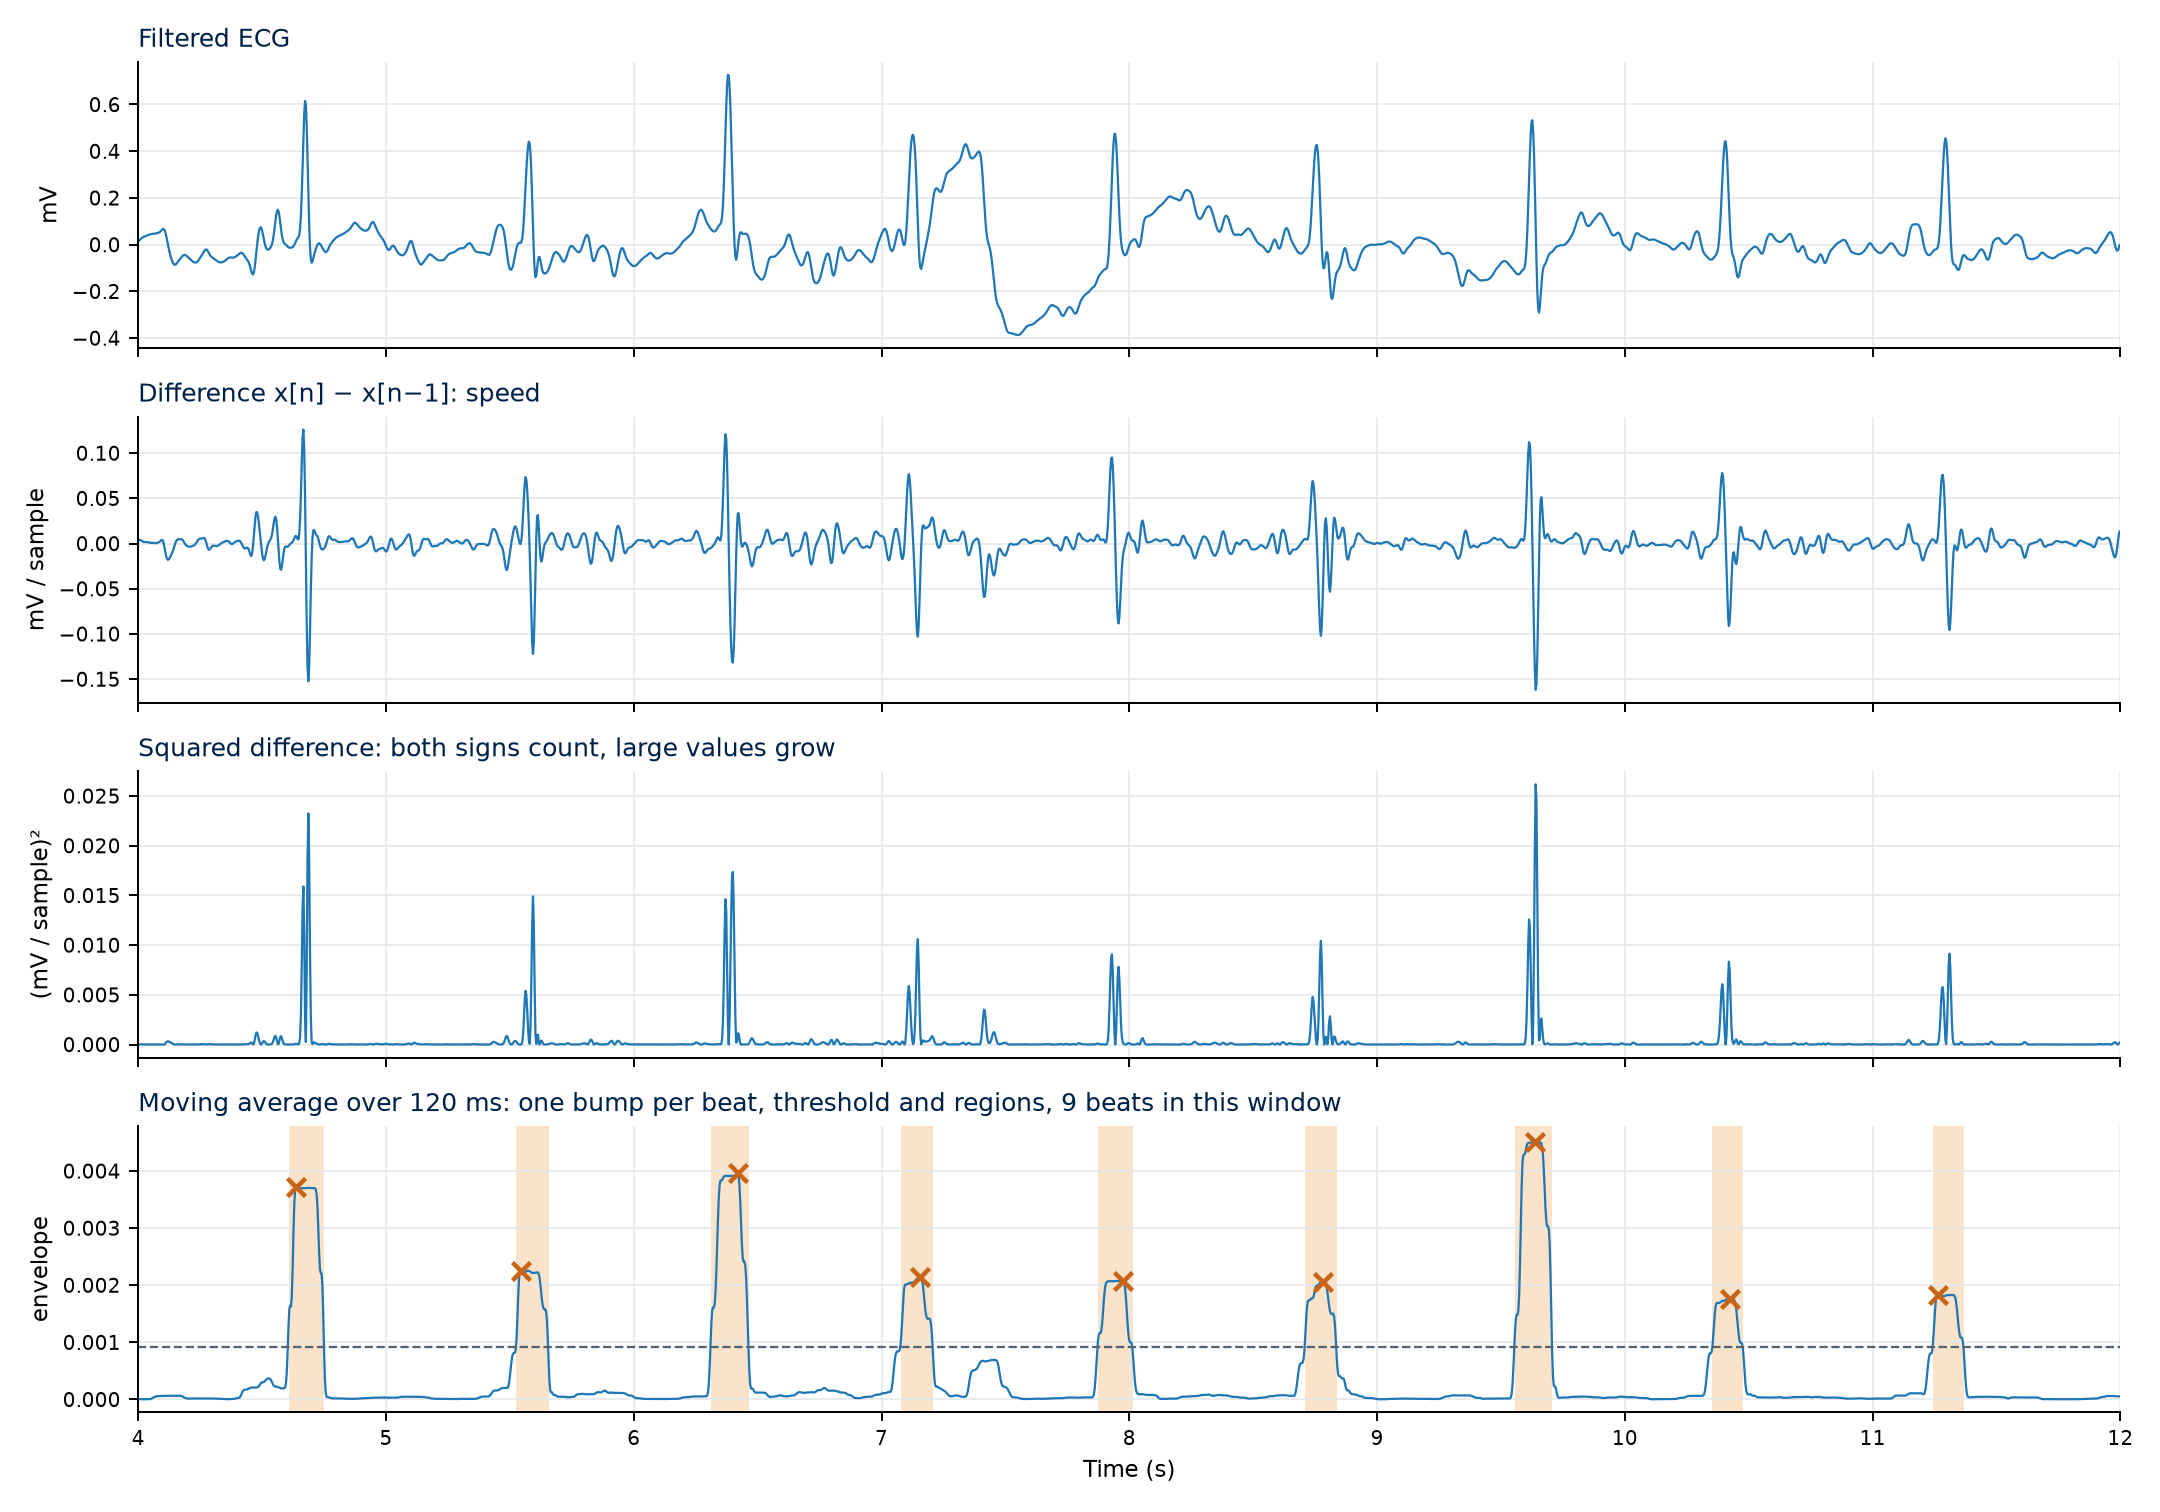
\includegraphics[width=\textwidth]{figures/step2_envelope.png}
  \caption{Step 2 on the same excerpt: filtered ECG, difference, squared difference, and the
  envelope with its threshold and regions. The swing that fooled step 1 is slow, so it almost
  vanishes in the difference; the envelope has one bump per beat, and the threshold now finds
  exactly the nine beats in the window.}
  \label{fig:step2}
\end{figure}

\paragraph{What it bought.} Most of the gap: beat agreement 0.72 to 0.92, heart rate MAE 52.6
to \SI{6.4}{bpm}. The RMSSD MAE also falls, 288 to \SI{218}{\milli\second}, but its P95 rises,
516 to \SI{648}{\milli\second}: on a few recordings a strong artefact now sets the threshold
for the whole recording.

\paragraph{Task 4B.} Write \texttt{differentiate} (the difference of neighbouring
samples, with a leading zero so the length is unchanged) and \texttt{envelope} (square, then a
centred moving average over the \SI{120}{\milli\second} window, rounded to an odd number of
samples). \emph{Deliver:} both functions with the checks passed, and the leaderboard line.

\begin{tcolorbox}[breakable, title=Specification: \texttt{differentiate(x)} and \texttt{envelope(d)}, colback=white, colframe=black!60]
\begin{description}[leftmargin=*, itemsep=2pt, font=\bfseries]
  \item[Given] \texttt{x}, the filtered ECG, a 1-D float array in mV; then \texttt{d}, the difference signal, with positive and negative spikes at every QRS; the setting \texttt{integration\_s} (0.12) above the function.
  \item[You may use] NumPy only (for the envelope, a convolution with a window of equal weights, or cumulative sums).
  \item[Return] \texttt{differentiate}: \texttt{d}, same length as \texttt{x}, with $d[n] = x[n] - x[n-1]$ for $n \geq 1$ and $d[0] = 0$. \texttt{envelope}: a non-negative array of the same length, at each sample the mean of $d^2$ over a window of \texttt{width} samples centred on it, where \texttt{width} is \texttt{integration\_s} $\times f_s$ rounded to an integer and made odd (37 samples at \SI{120}{\milli\second}); beyond the edges the signal counts as zero.
  \item[Checked by] the invented signal \texttt{[0, 1, 3, 1, 0]}, which must differentiate to \texttt{[0, 1, 2, -2, -1]}; and a reference envelope on your recording.
\end{description}
\end{tcolorbox}

\subsubsection{Step 3: locate the R peak on the ECG}
\nb{Task 4C}
\emph{Problem:} the envelope says roughly \emph{when} a beat happens, but its maximum is
smeared and sits after the R peak, and RR intervals are differences of these times.
Occasionally one beat still gives two regions. \emph{Idea:} in each candidate region, place
the beat at the maximum of the filtered ECG (the minimum for an inverted recording, chosen only
after inspecting the waveform), and keep no two beats closer than \SI{250}{\milli\second},
strongest first (Figure~\ref{fig:step3}). \emph{Caveats:} this rule can reject true fast beats
or keep strong artefacts.

\begin{figure}[htbp]
  \centering
  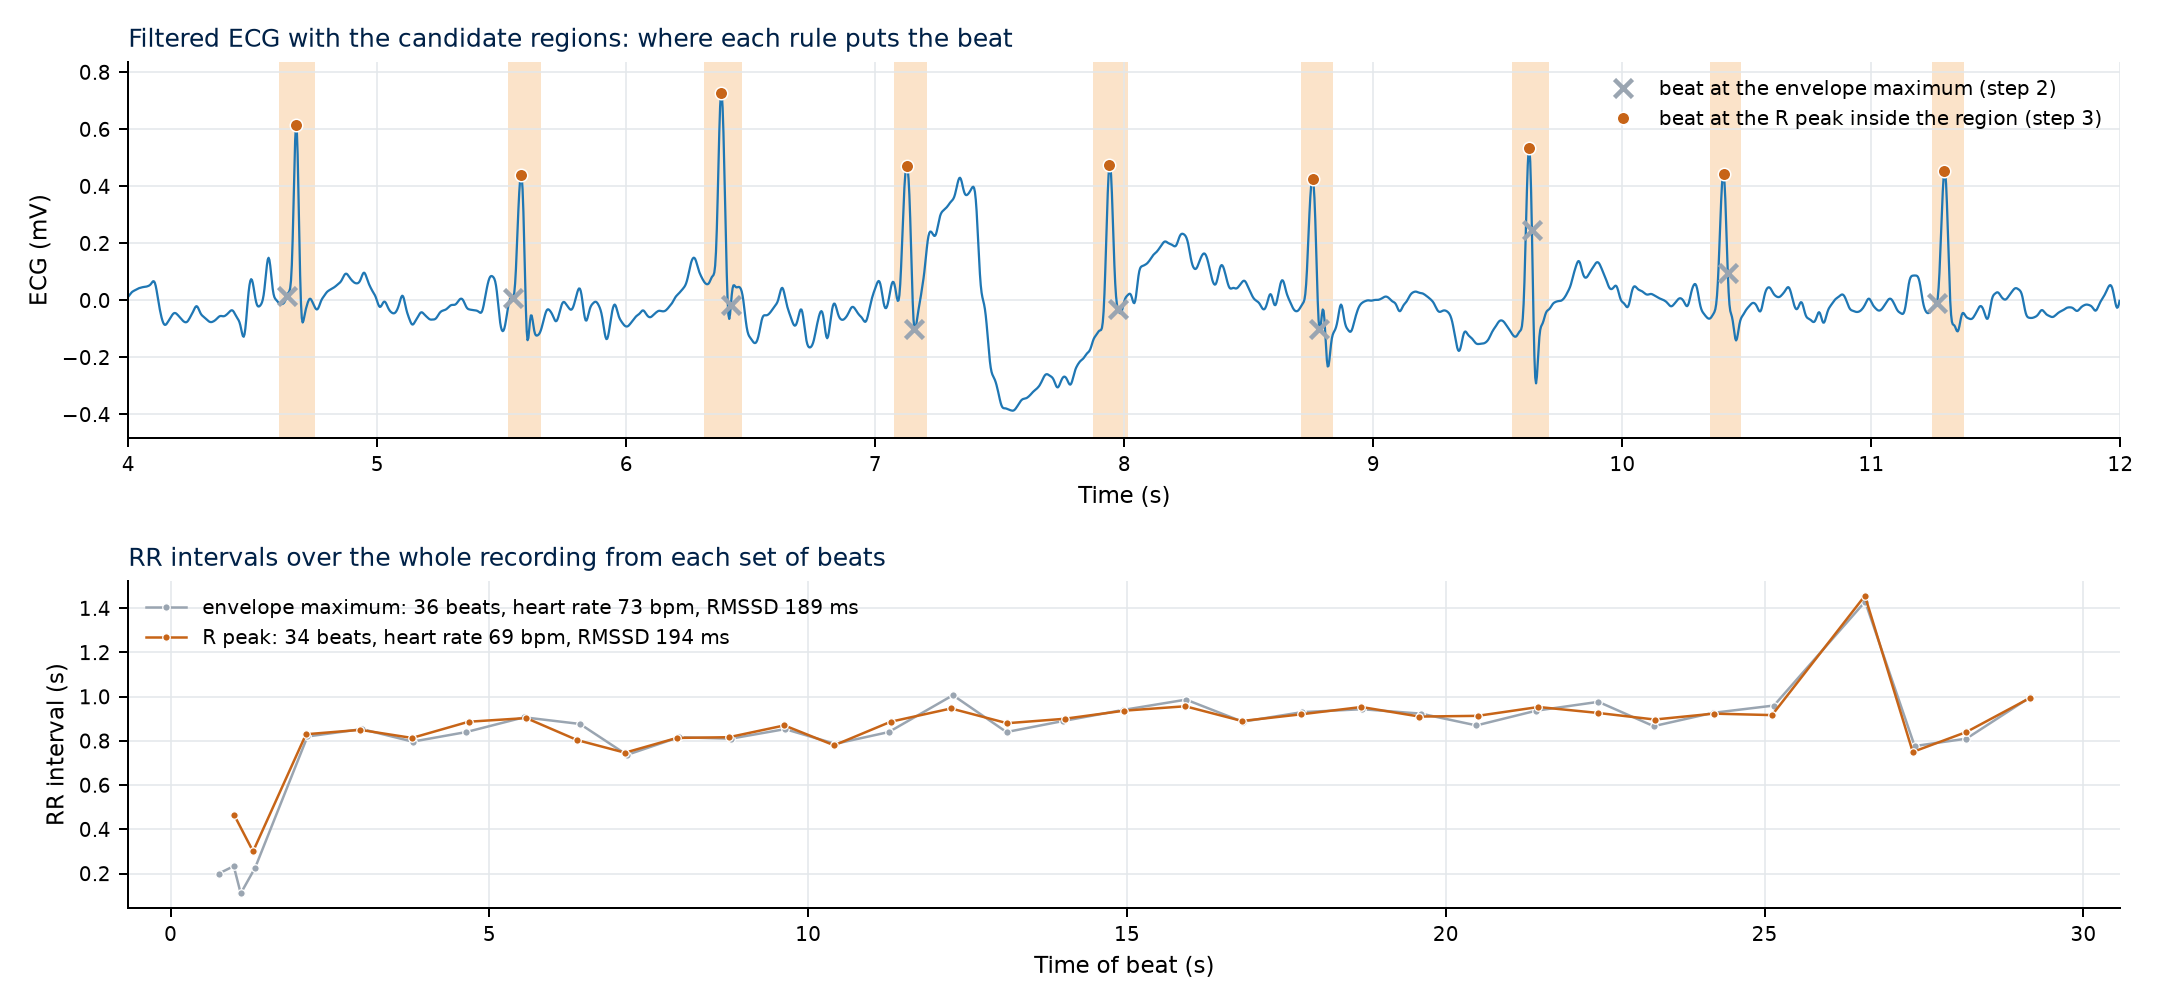
\includegraphics[width=\textwidth]{figures/step3_locate.png}
  \caption{Step 3 on \texttt{A00726}. Top: in each region, the beat at the envelope maximum
  (step 2) sits about \SI{40}{\milli\second} after the R peak, where step 3 puts it. Bottom: the
  RR intervals from each set of beats over the whole recording. The grey line zigzags where the
  orange one is smooth; the two large spikes, the artefact at \SI{1}{\second} and the missed
  beat at \SI{26}{\second}, are left for median imputation.}
  \label{fig:step3}
\end{figure}

\paragraph{What it bought.} Beat agreement hardly moves (0.92 to 0.91: the envelope maximum was
already within the \SI{100}{\milli\second} pairing tolerance), but the heart rate MAE falls
from 6.4 to \SI{5.1}{bpm} and the RMSSD MAE from 218 to \SI{194}{\milli\second}, because the
intervals are now measured between R peaks and not between smeared maxima.

\paragraph{Task 4C.} Write \texttt{locate}: one candidate per region, the highest
sample of the filtered ECG (the lowest for negative polarity); then go through the candidates
strongest first and keep one only if it is at least \SI{250}{\milli\second} from every beat
already kept. \emph{Deliver:} the function with the checks passed, and the leaderboard line.

\begin{tcolorbox}[breakable, title=Specification: \texttt{locate(ecg, starts, stops)}, colback=white, colframe=black!60]
\begin{description}[leftmargin=*, itemsep=2pt, font=\bfseries]
  \item[Given] \texttt{ecg}, the filtered ECG in mV; \texttt{starts} and \texttt{stops}, integer arrays of equal length in time order, region $k$ being \texttt{ecg[starts[k]:stops[k]]}, the regions disjoint, each meant to hold one beat but occasionally two regions on one beat. Inside the function \texttt{score} is defined: \texttt{ecg} for positive polarity, \texttt{-ecg} for negative, so the beat is always the highest sample of \texttt{score}. The settings \texttt{polarity} and \texttt{min\_separation\_s} (0.25) are above the function.
  \item[You may use] \texttt{highest\_in\_regions(signal, starts, stops)}, supplied in the detector v1 cell, which returns the highest sample of each region; Python's sorting; NumPy.
  \item[Return] a 1-D integer array of beat indices in time order: one candidate per region, with every candidate closer than \texttt{min\_separation\_s} $\times f_s$ samples to a \emph{stronger} kept candidate removed. Going through the candidates strongest first guarantees that the stronger of two close candidates is the one kept.
  \item[Checked by] an invented signal with peaks of height 5, 6 and 3 at samples 100, 150 and 500, which must give \texttt{[150, 500]}; and a reference implementation on your recording.
\end{description}
\end{tcolorbox}

\subsection{Median imputation: correcting the HRV estimate}
\label{sec:impute}
\nb{3.4, Task 4D}
\emph{Problem:} after the three steps of Section~\ref{sec:qrs} a few beats are still wrong: an
artefact taken for a beat, or a small QRS that never crossed the threshold. Such an error
barely affects the heart rate, but it does affect RMSSD, because one missed beat creates two
large successive differences in a row.
\emph{Idea:} a peak-finding or QRS-searching detector is agnostic of rhythm. It detects each
beat from local features only, which makes it sensitive to noise: an artefact right after a
beat becomes two beats in rapid succession, and a small QRS becomes none. Yet a human heart
beats with a specific rhythm, and the beats around a doubtful one say a lot about whether it is
real. Median imputation adds that rhythm. The median RR interval is the recording's
typical interval, and a few wrong beats barely move it. Going through the beats in time order,
a beat closer than $0.6\times$ the median RR to the last kept beat is dropped as an extra, and
a gap longer than $1.6\times$ the median RR is split evenly into round(gap / median RR)
intervals, inserting beats. If the median rate is outside \SIrange{30}{200}{bpm}, most beats are
wrong and the median cannot be trusted, so nothing is changed. On the recording in Figure~\ref{fig:recipe}
it removes the artefact and fills the gap: RMSSD falls from 194 to \SI{67}{\milli\second} while
the heart rate stays at \SI{69}{bpm}. The reference is not corrected, so where it has an error of its own, correcting
ours moves us away from it. \emph{Caveats:} inserted beats are invented and evenly
spaced, so they pull RMSSD down; a genuine premature beat, as in Section~1's \texttt{O}
example, is ``corrected'' away; and in atrial fibrillation the irregularity is the physiology,
not noise. The rule is a teaching version of two established ideas: QRS detectors search back
for a missed beat when no beat has been found within about one and a half times the average RR
interval~\cite{pan1985qrs, hamilton1986qrs}, and HRV editing identifies extra and missed beats
as intervals that deviate from the local distribution and corrects them by merging or splitting
intervals~\cite{berntson1990artifact}. The current standard, used by Kubios and by NeuroKit2's
\texttt{signal\_fixpeaks}, classifies beats with time-varying thresholds on the successive
differences~\cite{lipponen2019artefact}. The rule used here is the simplest member of that
family, and that is why it was chosen for teaching: it fits in a few lines, and every decision
it makes can be read off the RR plot. The factors 0.6 and 1.6 are teaching choices, not taken
from any of these papers.

\begin{figure}[tbp]
  \centering
  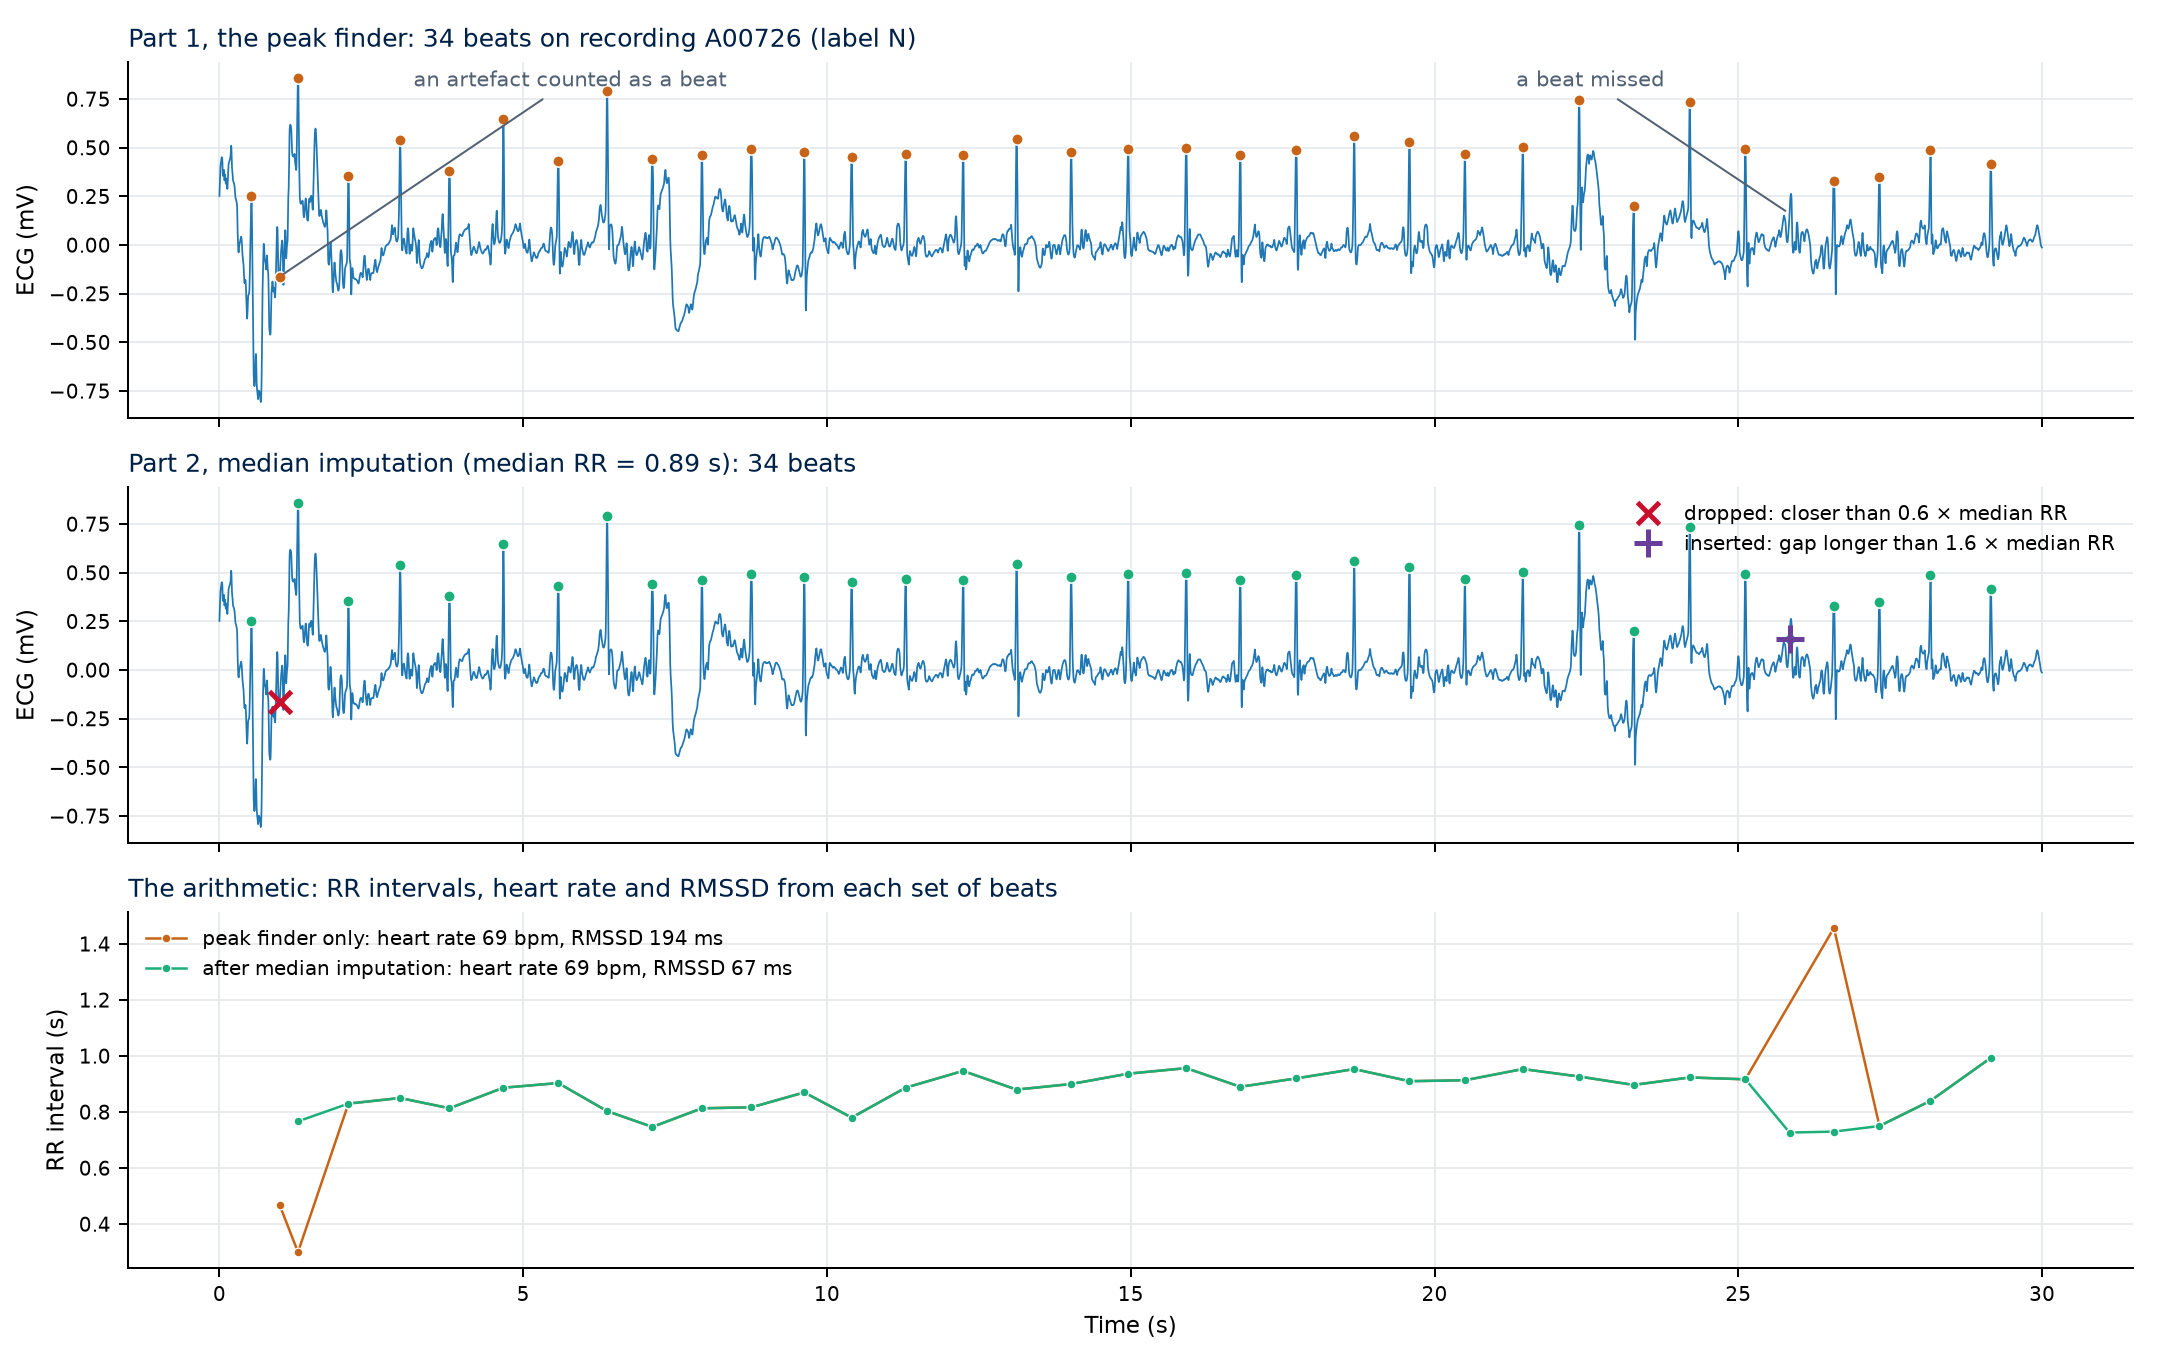
\includegraphics[width=\textwidth]{figures/recipe.png}
  \caption{Median imputation on an \texttt{N} recording. Top: the peak finder's beats; it counts an
  artefact at \SI{1.0}{\second} and misses a beat at \SI{25.8}{\second}. Middle: the
  median imputation, with a median RR of \SI{0.89}{\second}, drops the first (closer than $0.6\times$ the
  median RR to the previous beat) and inserts the second (a gap longer than $1.6\times$ the
  median RR). Bottom: the RR intervals and the numbers from each set of beats. The heart rate
  does not change; RMSSD falls from 194 to \SI{67}{\milli\second}.}
  \label{fig:recipe}
\end{figure}

\paragraph{What it bought.} The RMSSD MAE falls from 194 to \SI{146}{\milli\second} and its P95
from 604 to \SI{393}{\milli\second}; the heart rate P95 from 32 to \SI{28.5}{bpm}. Beat
agreement slips from 0.91 to 0.90: where the reference has a missed or extra beat of its own, our
corrected beats no longer pair with it.

\paragraph{Task 4D.} Write \texttt{correct}: the median RR of the beats, then
the walk in time order with its two rules, drop when closer than 0.6~$\times$ the median, fill
when further than 1.6~$\times$; the rate guard is supplied. \emph{Deliver:} the function with
the checks passed, and the leaderboard line.

\begin{tcolorbox}[breakable, title=Specification: \texttt{correct(beats)}, colback=white, colframe=black!60]
\begin{description}[leftmargin=*, itemsep=2pt, font=\bfseries]
  \item[Given] \texttt{beats}, a 1-D integer array of sample indices in time order from detector 4C, usually 30 to 60 per recording, occasionally with an extra one (an artefact) or a missing one (a small QRS); the settings \texttt{correct\_short} and \texttt{correct\_long} (0.6 and 1.6) above the function. The rate guard, the walk through the beats and the insertion of evenly spaced beats are supplied; you write the four quantities the rule needs.
  \item[You may use] NumPy only.
  \item[Return] a 1-D integer array in time order, the beats with every extra one dropped and every gap filled. \texttt{median\_rr} is the median RR interval in samples; for each beat, \texttt{gap} (supplied) is its distance to the last kept beat; \texttt{too\_close} is whether the gap is shorter than \texttt{correct\_short} $\times$ \texttt{median\_rr}; \texttt{too\_far} is whether it is longer than \texttt{correct\_long} $\times$ \texttt{median\_rr}; \texttt{k} is the number of intervals the gap should hold, \texttt{gap / median\_rr} rounded to an integer.
  \item[Checked by] the invented beats \texttt{[0, 300, 600, 900, 1500, 1800, 1850, 2100]} (median RR 300), which must give \texttt{[0, 300, 600, 900, 1200, 1500, 1800, 2100]}; and a reference implementation on \texttt{A00726}.
\end{description}
\end{tcolorbox}

% ____________________________________________________________________________
\needspace{10\baselineskip}
\section{Classifying rhythms with ECG features}
\nb{Section 4}

In clinical practice, wearable ECGs are often used to detect heart problems that a clinic
visit might miss. Atrial fibrillation is the main one: it often comes and goes, is often
silent, raises the risk of stroke about fivefold~\cite{wolf1991af}, and can be treated once it
is found. So people record short strips at home, by the million, and no cardiologist can read
them all. In this section we use the two features of Section~3, heart rate and RMSSD, together
with the other ECG features a library extracts, to predict the rhythm of each recording:
\texttt{N}, \texttt{A}, \texttt{O} or \noise. That prediction is the triage: likely AF goes
to a clinician, noise is recorded again, normal is filed. The label is a screening flag, not a
diagnosis. The 2017 challenge that produced this dataset was set up for exactly this task, by
the makers of such a device~\cite{clifford2017af}.

\subsection{NeuroKit2 ECG features}
\nb{4.1}
\paragraph{From two features to the full set.} In Section~3 you extracted two features,
heart rate and RMSSD, with a detector you built. They are two of many. Once the beats are
known, and the P, Q, S and T waves around each of them, a library can measure a whole family of
numbers from the same recording (Table~\ref{tab:features}): how the RR intervals around each
beat compare with one another; how far apart the waves of a beat are in time and in amplitude,
which is the shape of the beat rather than its timing; the 25 HRV features of
Table~\ref{tab:hrv}, which generalise RMSSD; and one number for the quality of the signal.
Section~2 showed that RMSSD alone already separates \texttt{N} from \texttt{A} to a useful
degree, but \texttt{O} overlaps both and \noise\ is scattered, so no single threshold will do.
A classifier combines all 54 and draws the boundary itself. The route is interpretable, you can
ask which features the classifier relies on, and it learns from about 1,400 labelled
recordings. Its price is that every new problem needs new expertise and new features. Lab~2
asks what happens when nobody designs them.

\paragraph{How they are extracted.} \texttt{extract\_feature} runs the reference pipeline on a
whole recording (\texttt{ecg\_clean}, then \texttt{ecg\_peaks}, no correction), locates the P,
Q, S and T waves around each beat with \texttt{ecg\_delineate}, and returns the 54 numbers of
Table~\ref{tab:features}. It runs without visual review: that is what makes 2,000 recordings
feasible, and also the risk: nobody checks the beats.

\begin{table}[htbp]
\centering
\singleTableRowHeight
\small
\begin{tabular}{>{\raggedright\arraybackslash}p{3.2cm} c >{\raggedright\arraybackslash}p{9cm}}
\tableHeaderStart
\tableHCell{Family} & \tableHCell{Count} & \tableHCell{Features} \\
\tableHeaderEnd
R-peak timing & 8 & R amplitude (\texttt{a\_R}); the RR intervals before, after and two after
  each beat (\texttt{RR0}, \texttt{RR1}, \texttt{RR2}) and their mean (\texttt{RRm}); the ratios
  \texttt{RR0/RR1}, \texttt{RR2/RR1}, \texttt{RRm/RR1} \\
Wave shape & 20 & time between wave peaks: \texttt{t\_PR}, \texttt{t\_QR}, \texttt{t\_RS},
  \texttt{t\_RT}, \texttt{t\_PQ}, \texttt{t\_PS}, \texttt{t\_PT}, \texttt{t\_QS}, \texttt{t\_QT},
  \texttt{t\_ST}; amplitude difference between wave peaks: \texttt{a\_PQ}, \texttt{a\_QR},
  \texttt{a\_RS}, \texttt{a\_ST}, \texttt{a\_PS}, \texttt{a\_PT}, \texttt{a\_QS}, \texttt{a\_QT},
  and the ratios \texttt{a\_ST/a\_QS}, \texttt{a\_RS/a\_QR} \\
Heart rate variability & 25 & \textbf{MeanNN} (the heart rate is $60\,000 / \text{MeanNN}$),
  \textbf{RMSSD}, and the other 23 time-domain features of Table~\ref{tab:hrv}: SDNN, CVNN,
  MadNN, MCVNN, IQRNN, Prc20NN, Prc80NN, MedianNN, MinNN, MaxNN, SDANN1/2/5, SDNNI1/2/5, SDSD,
  CVSD, SDRMSSD, pNN50, pNN20, HTI, TINN \\
Signal quality & 1 & \texttt{SQI}, NeuroKit2's quality index \\
\hline
\end{tabular}
\caption{The 54 features of \texttt{extract\_feature}. Every one is computed per beat and
averaged over the recording, except the HRV features and the SQI, which are computed over the
whole recording. In bold, the two you computed in Section~3.}
\label{tab:features}
\end{table}
\FloatBarrier

\subsection{Training a RandomForest with the features}
\nb{4.2, Task 5}
We will train a RandomForest~\cite{breiman2001rf} of 100 trees on the 54 features and use it
to predict the rhythm of unseen ECG recordings. The data are already prepared: the feature
table (\texttt{ECG\_feature.pkl}) was computed in advance for all 2,000 recordings, and the
recordings are split 70\% / 15\% / 15\% into training (1,400), validation and test sets with
\texttt{random\_state=42}, the same split as Lab~2. Because the classes are unbalanced, the
evaluation metric is the \emph{macro-averaged F1}: the mean of the four classes' F1 scores, so
that each class counts equally. A reference training gives the scores in
Table~\ref{tab:classifier}: accuracy 0.79 and a macro F1 of 0.64 on the test set.

\begin{table}[htbp]
\centering
\singleTableRowHeight
\small
\begin{tabular}{l c c c c}
\tableHeaderStart
\tableHCell{Class} & \tableHCell{Precision} & \tableHCell{Recall} & \tableHCell{F1} & \tableHCell{Support} \\
\tableHeaderEnd
\texttt{N} normal sinus rhythm & 0.85 & 0.92 & 0.88 & 173 \\
\texttt{A} atrial fibrillation & 0.71 & 0.73 & 0.72 & 30 \\
\texttt{O} other rhythm & 0.70 & 0.63 & 0.66 & 86 \\
\noise\ too noisy & 0.67 & 0.18 & 0.29 & 11 \\
Macro average & 0.73 & 0.62 & \textbf{0.64} & 300 \\
\hline
\end{tabular}
\caption{The RandomForest on the 300 test recordings. Accuracy is 0.79; the macro F1 of 0.64
(0.68 on the validation set) is the number Lab~2 compares against.}
\label{tab:classifier}
\end{table}

\begin{figure}[htbp]
  \centering
  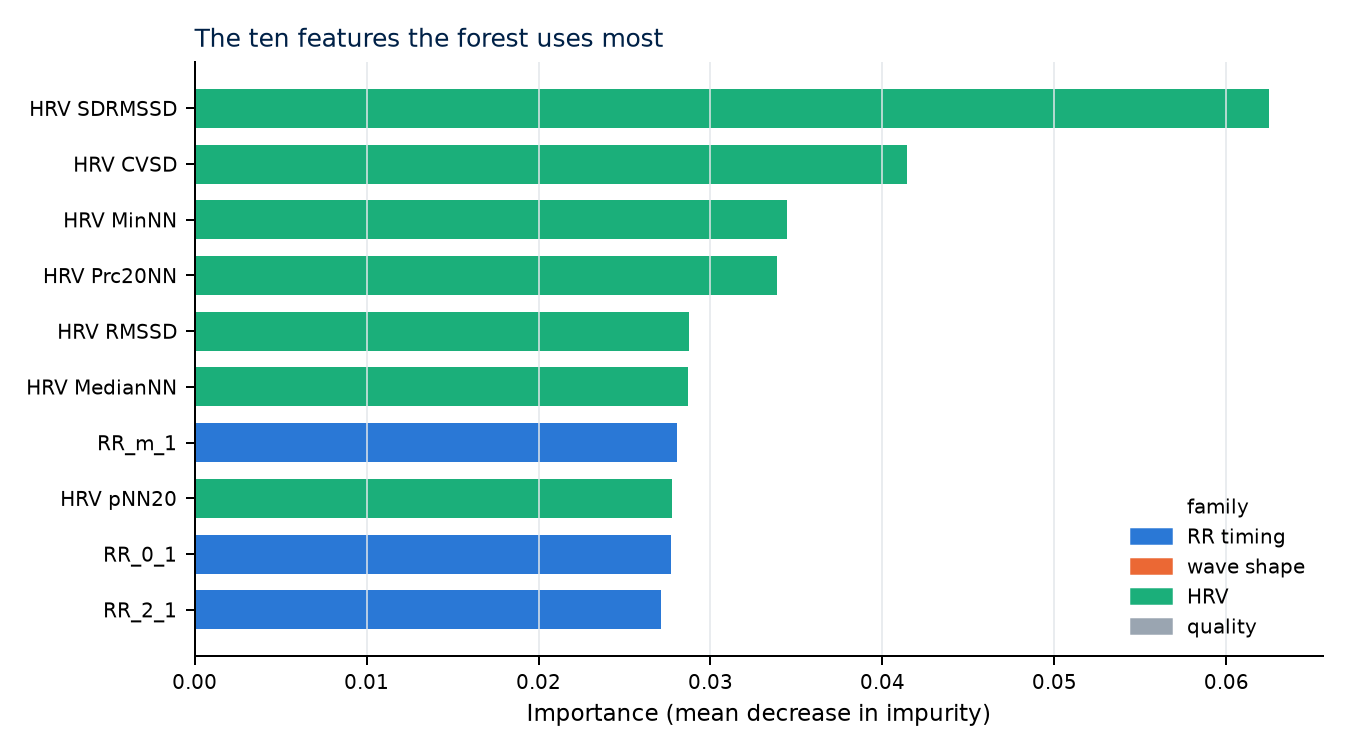
\includegraphics[width=0.8\textwidth]{figures/classifier.png}
  \caption{The ten features the forest uses most, coloured by family; all ten are rhythm
  features.}
  \label{fig:classifier}
\end{figure}

\paragraph{Analysing the result.} Which features does the forest rely on
(Figure~\ref{fig:classifier})? Half of the
importance sits in the 25 HRV features and another fifth in the 8 RR-timing features; the ten
most used are all rhythm features, led by SDRMSSD, CVSD and RMSSD, which measure how much the
intervals vary. That agrees with the definition of atrial fibrillation in Section~1: the
rhythm is \emph{irregularly irregular}, so what separates \texttt{A} is the intervals, not the
waves.

\paragraph{Task 5.} Write \texttt{train\_forest}: a \texttt{StandardScaler}
fitted on the training set only, and a \texttt{RandomForestClassifier} of 100 trees
(\texttt{random\_state=42}) fitted on the scaled training features; and \texttt{predict}:
scale new features with the same scaler and return the model's predictions. The notebook checks
your test-set predictions against a reference, prints the classification reports and plots the
ten features the forest uses most. \emph{Deliver:} both functions with the check passed; the
test report; and your test macro F1, written down for Lab~2.

\begin{tcolorbox}[breakable, title=Specification: \texttt{train\_forest(x\_train, y\_train)} and \texttt{predict(scaler, model, x)}, colback=white, colframe=black!60]
\begin{description}[leftmargin=*, itemsep=2pt, font=\bfseries]
  \item[Given] \texttt{x\_train}, a 2-D float array of 1,400 rows (recordings) $\times$ 54 columns (features), unscaled, with ranges that differ by orders of magnitude between columns; \texttt{y\_train}, an integer array of 1,400 class codes (0 to 3). For \texttt{predict}: the two fitted objects and \texttt{x}, $n \times 54$ unscaled features.
  \item[You may use] \texttt{StandardScaler} and \texttt{RandomForestClassifier}, imported at the top of the cell; their documentation gives the arguments.
  \item[Return] \texttt{train\_forest}: \texttt{(scaler, model)}, a scaler fitted on \texttt{x\_train} only (each column centred and scaled by the training set's mean and standard deviation) and a forest of 100 trees with \texttt{random\_state=42} fitted on the scaled \texttt{x\_train} and \texttt{y\_train}. \texttt{predict}: an integer array of $n$ predicted class codes, from \texttt{x} scaled with the same scaler.
  \item[Checked by] the reference model's predictions on the 300 test recordings, which yours must match exactly.
\end{description}
\end{tcolorbox}

\paragraph{Carry forward.} From a raw strip to a screening label, every step was designed by a
person: the filter band, the envelope window, the median-RR rule, the 54 features. The result
is interpretable and learns from 1,400 recordings, and it is only as good as the features and
the beats under them. Lab~2 trains networks on the same recordings and the same split, with
no designed features, and compares them with your macro F1.


% ____________________________________________________________________________
\section*{Submitting your work}
\addcontentsline{toc}{section}{Submitting your work}
Save the notebook with your code and plots. Restart the kernel and run all cells
to check that your work is reproducible, and keep your test macro F1 from Section~4 for Lab~2.

\paragraph{Acknowledgement.} The learning sequence derives from the CWM Wearable Technology
practical by Mauricio Villarroel, with detector material credited to Gari Clifford and Mauricio
Villarroel~\cite{villarroel_cwm}. The current \SI{300}{\hertz} implementation is a teaching
adaptation, not a numerical reproduction of that detector.


\backmatter
\listofreferences

\end{document}
